\chapter{Podstawy}

W tym rozdziale zostaną omówione wszystkie ważniejsze pojęcia, którymi będziemy się od tej pory posługiwać. Przedstawimy przede wszystkim pojęcie \textbf{grafu} i sposoby jego reprezentacji w algorytmach, które będziemy omawiać w późniejszej części pracy. Przedyskutujemy postawiony przed nami problem wyszukiwania \textbf{najkrótszych ścieżek} w rzeczywistych sieciach drogowych, a także przyjrzymy się dokładnie własnościom, z jakich przyjdzie nam niejednokrotnie skorzystać podczas analizy kolejnych rozwiązań tego problemu. Na końcu tego rozdziału przedstawimy algorytm Bellmana-Forda jako podstawową ideę rozwiązywania tego typu problemów, zastanowimy się nad tym co można w nim usprawnić, aby uzyskiwać rozwiązania problemu w znacznie krótszym czasie.

\section{Grafy w sieciach drogowych}

\textbf{Grafem} będziemy nazywać taką parę $G = \left( V, E \right) $, gdzie każde $v \in V$ jest \textbf{wierzchołkiem} tego grafu, zaś każdy element $e \in E$ jest jego \textbf{krawędzią}, łączącą dowolne dwa wierzchołki.

W naszym przypadku krawędzie ($E$) grafu będziemy rozumieć jako dowolny odcinek drogi na jezdni między dwoma dowolnie wybranymi punktami $v_{p}$ oraz $v_{k}$, gdzie przez $v_{i}$ dla $i \in \left\{ 1, \ldots, \left| V \right| \right\}$ będziemy od tej pory oznaczać dowolny wierzchołek w grafie $G$ (w odniesieniu do rzeczywistego ruchu drogowego może to być skrzyżowanie, dowolny punkt drogi na wysokości jakiegoś specyficznego budynku, miejsca wystąpienia znaku drogowego itp.). Taką krawędź będziemy zwykle oznaczać przez $e_{pk}$, gdzie kolejność wypisania indeksów określa nam zwrot danego łuku. Stosowanie grafowej reprezentacji w odniesieniu do sieci dróg determinuje w pewnym stopniu właściwości grafu z jakim będziemy mieli do czynienia. Nie będzie w nim na pewno krawędzi, których \textbf{koszt} jest mniejszy lub równy zero. W ogólności nie będziemy także mogli nic powiedzieć o acykliczności grafu, ani rozstrzygnąć, czy będziemy pracować na grafach skierowanych czy nie - zdecydowana większość rozważanych sieci drogowych posiada jednak w swojej topologii liczne cykle, a także wiele dróg jednokierunkowych i właśnie na taki model grafu - skierowany z cyklami - się zdecydujemy.

Każda krawędź w grafie posiada swoją \textbf{wagę}, podobnie jak każda droga z punktu $v_{p}$ do $v_{k}$ ma zdefiniowaną odległość między tymi dwoma punktami, wyrażoną w dowolnych jednostkach długości. Aby uprościć nasz model grafu założymy, że \textbf{koszt} (waga) każdego łuku \footnote{w odniesieniu do połączeń pomiędzy węzłami w grafie $G = \left( V, E \right) $ będziemy wymiennie stosować nazwy: krawędź, łuk, połączenie.} będzie wyrażony przez jedną liczbę naturalną, będącą odzwierciedleniem odległości między punktami, które dana krawędź $e \in E$ łączy. W rzeczywistych warunkach drogowych takie połączenie mogłoby posiadać cały szereg atrybutów takich jak np. intensywność ruchu ulicznego, rodzaj nawierzchni, nachylenie terenu, ograniczenia prędkości na danym odcinku drogi, które miałyby bezpośredni wpływ na wybór najkrótszej ścieżki od punktu $v_{p}$ do $v_{k}$, a które my w swoich rozważaniach, dla zachowania ich prostoty, pominiemy.

\section{Reprezentacje grafu}

W informatyce istnieje kilka sposobów na efektywne przedstawienie struktury grafu. Jak później pokażemy, wybór ten w znaczny sposób może wpłynąć na efektywność algorytmów wyszukiwania najkrótszych ścieżek, zarówno na ich złożoność czasową jak i pamięciową. W niniejszym podrozdziale pokażemy trzy różne podejścia do problemu przedstawienia grafu jako struktury w programie, gdzie pierwsze z nich zakłada tworzenie dla grafu wejściowego \textbf{macierzy incydencji} - jednego z dwóch wariantów reprezentacji macierzowej grafu jakie będziemy rozróżniać.

\subsection{Macierz incydencji}

\textbf{Macierz incydencji} dla grafu $G = \left( V, E \right) $ jest to macierz o wymiarach $\left| V \right| \times \left| E \right|$, gdzie każda komórka jest zdefiniowana następująco:

\begin{equation}
	a_{ij}= \left\{ 
	\begin{array}{ll}
	-1 & \textrm{jeżeli krawędź $j$ wychodzi z wierzchołka $i$,}\\
	1 & \textrm{jeżeli krawędź $j$ wchodzi z wierzchołka $i$,}\\
	0 & \textrm{w przeciwnym wypadku}
	\end{array} \right.
\end{equation}

gdzie:

\begin{equation}
	\begin{array}{lll}
	i & \in & \left\{ 1, \ldots, \left| V \right| \right\} \textrm{,} \\
	j & \in & \left\{ 1, \ldots, \left| E \right| \right\} \textrm{.}
	\end{array}
\end{equation}

Innymi słowy każde połączenie w grafie między dwoma wierzchołkami $v_{p}$ i $v_{k}$ jest traktowane jako takie, które uaktywniamy, pobierając jedną jednostkę "energii" (stąd w macierzy na odpowiednim miejscu wartość $-1$), którą następnie przekazujemy do docelowego wierzchołka $v_{k}$ (co odnotowujemy w macierzy wartością $+1$).

\begin{figure}[!htbp]
	\centering
	\begin{subfigure}[b]{0.45\textwidth}
		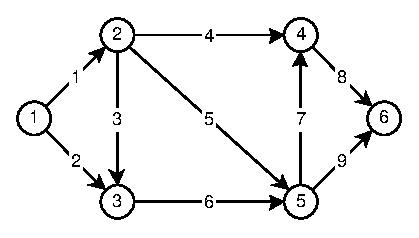
\includegraphics[width=\textwidth]{Chapter_I/1/1_1a.eps}
		\caption{}
	\end{subfigure}%
	%add desired spacing between images, e. g. ~, \quad, \qquad, \hfill etc.
	%(or a blank line to force the subfigure onto a new line)
	\qquad
	\begin{subfigure}[b]{0.45\textwidth}
		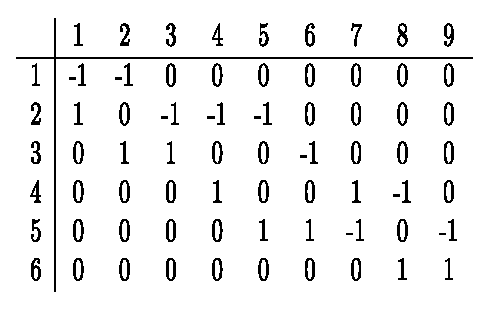
\includegraphics[width=\textwidth]{Chapter_I/1/1_1b.eps}
		\caption{}
	\end{subfigure}
	\caption{\textbf{Macierz incydencji} \textbf{(a)} Graf skierowany $G = \left( V, E \right)$ z identyfikatorami węzłów $1-6$ i łuków $1-9$ (dla znanych identyfikatorów łuków będziemy stosować oznaczenie $e_{i}$ zamiast $e_{pk}$). \textbf{(b)} Macierz incydencji $ \left| V \right| \times \left| E \right| $ grafu $G$.}\label{fig:incidenceMatrix}
\end{figure}

Operacje, jakie będziemy chcieli - jak się później okaże - wykonywać na tak zdefiniowanej macierzy (i na każdej następnej strukturze z tego podrozdziału) to procedury wyszukiwania wszystkich bezpośrednich następników danego węzła $v_{i}$ (oznaczać będziemy taki zbiór za pomocą symbolu $A \left( i \right) $) i odnajdywania każdego takiego łuku, wychodzącego z danego węzła do wszystkich $v_{k} \in A \left( i \right) $. Dla pierwszego podejścia:

\begin{myitemize}
	\item koszt identyfikacji wszystkich łuków jest ściśle powiązany z ilością krawędzi w grafie - wystarczy, że dla wierzchołka $v_{i}$ przejrzymy cały jeden wiersz o indeksie $i$, aby odnaleźć identyfikatory wszystkich krawędzi, bezpośrednio wychodzących z danego wierzchołka (wszystkie komórki o wartości mniejszej od zera). Możemy ograniczyć ilość potrzebnych skanowań poprzez wprowadzenie licznika krawędzi wychodzących, lecz w najgorszym możliwym przypadku takie skanowanie wciąż będzie wymagało $O \left( m \right)$ porównań, gdzie $m$ to oczywiście liczba krawędzi w grafie.
	\item Koszt wyszukiwania wszystkich następników węzła $v_{i}$, obejmuje koszt wyszukania wszystkich łuków, prowadzących do tych wierzchołków oraz odnalezienie ich identyfikatorów - co dla każdego odnalezionego łuku $e_{j}$ zmusza nas do przeszukania wszystkich elementów macierzy, znajdujących się w tej samej, $j$'tej kolumnie. Takich kolumn, jak wspomnieliśmy wcześniej, będzie $ \left| A \left( i \right) \right| $, przeszukanie każdej $j$'tej kolumny wymagać będzie, w najgorszym przypadku, $n-1$ porównań dla każdej z nich tak więc ostatecznie otrzymujemy $O \left( \left| A \left( i \right) \right| \cdot n \right)$ dla wyszukiwania wszystkich następników węzła $v_{i}$ (wraz z wyszukiwaniem łuków $O \left( m + \left| A \left( i \right) \right| \cdot n \right)$).
\end{myitemize}

\subsection{Macierz sąsiedztwa}

Oprócz macierzowej reprezentacji typu wierzchołek-krawędź możliwe jest także reprezentowanie struktury grafu za pomocą macierzy typu wierzchołek-wierzchołek. \textbf{Macierz sąsiedztwa} dla grafu $G = \left( V, E \right) $ jest to macierz o wymiarach $\left| V \right| \times \left| V \right|$, gdzie wartość każdej komórki jest zdefiniowana następująco:

\begin{equation}
	b_{ij}= \left\{ 
	\begin{array}{ll}
	1 & \textrm{jeżeli istnieje ścieżka z wierzchołka $v_{i}$ do $v_{j}$,}\\
	0 & \textrm{w przeciwnym wypadku}
	\end{array} \right.
\end{equation}


O ile, w przypadku takiego przedstawienia grafu, jesteśmy w stanie uzyskać informacje o wszystkich bezpośrednich następnikach dowolnego węzła w czasie liniowym (dla węzła $v_{i}$ wystarczy przeszukać wiersz o indeksie $i$) to macierz w takiej postaci nie niesie ze sobą istotnych informacji o krawędziach grafu - takich, które umożliwiłyby ich szybką identyfikację, nie zmuszając nas do ponownego przeglądania wszystkich krawędzi grafu w poszukiwaniu łuku, który ma swój początek i koniec w - danych nam przez macierz - wierzchołkach. Umiejętność szybkiej identyfikacji takich krawędzi będzie nam w późniejszych rozważaniach nieodzowna, jako że chcemy się skupić na wyszukiwaniu najkrótszych ścieżek, gdzie kluczowych informacji dla tego problemu będziemy szukać właśnie w krawędziach między wierzchołkami. Załóżmy, że każda krawędź będzie określana za pomocą trzech cech: wierzchołka startowego, końcowego oraz odległości między tymi dwoma punktami. Zauważmy, że w takim przypadku wszystkie informacje o krawędzi możemy umieścić bezpośrednio w macierzy sąsiedztwa, zastępując starą definicję nową: 

\begin{equation}
	b_{ij}= \left\{ 
	\begin{array}{ll}
	$ d ( i, j ) $ & \textrm{jeżeli istnieje ścieżka z wierzchołka $v_{i}$ do $v_{j}$,}\\
	0 & \textrm{w przeciwnym wypadku}
	\end{array} \right.
\end{equation}

gdzie przez $ d \left( i,j \right) $ zwykle będziemy oznaczać długość ścieżki (odległość między wierzchołkami, które łączy). Takie podejście pozwala nam na nie tworzyć dodatkowych struktur, przechowujących informacje o krawędziach. Jeżeli chcielibyśmy wzbogacać naszą strukturę krawędzi wygodniej (a także bezpieczniej) zamiast wartości $d \left( i,j \right)$ w danych komórkach $b_{ij}$ będzie wstawić numer identyfikatora danej krawędzi. Zapewni nam to dodatkowo jednoznaczność w przypadku chęci identyfikacji krawędzi (zwróćmy uwagę, że oba łuki, wchodzące do węzła $v_{4}$ mają ten sam koszt $ d \left( 2, 4 \right) = d \left( 5, 4 \right) = 2$, co uniemożliwia nam ich rozróżnienie).

\begin{figure}[!htbp]
	\centering
	\begin{subfigure}[b]{0.45\textwidth}
		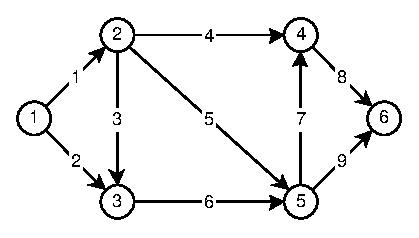
\includegraphics[width=\textwidth]{Chapter_I/2/1_2a.eps}
		\caption{}
	\end{subfigure}
	\qquad
	\begin{subfigure}[b]{0.09\textwidth}
		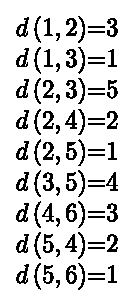
\includegraphics[width=\textwidth]{Chapter_I/2/1_2b.eps}
		\caption{}
	\end{subfigure}
	\qquad
	\begin{subfigure}[b]{0.35\textwidth}
		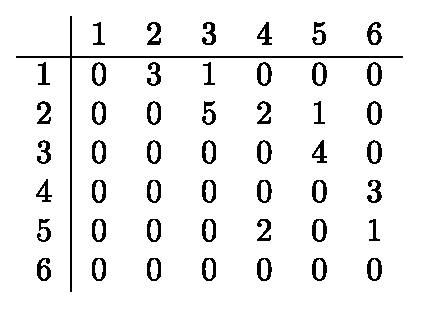
\includegraphics[width=\textwidth]{Chapter_I/2/1_2c.eps}
		\caption{}
	\end{subfigure}
	\caption{\textbf{Macierz sąsiedztwa} \textbf{(a)} Graf skierowany $G = \left( V, E \right)$ z identyfikatorami węzłów $1-6$ i łuków $1-9$. \textbf{(b)} Wagi/koszty łuków grafu $G$. \textbf{(c)} Macierz sąsiedztwa $ \left| V \right| \times \left| V \right| $ grafu $G$. Dla każdej wagi łuku $ d \left( v_{p}^{ID}, v_{k}^{ID} \right) = c$ odpowiednie komórki na przecięciu wiersza o numerze $v_{p}^{ID}$ i kolumny $v_{k}^{ID}$ mają wartość równą $c$, gdzie $v_{k}^{ID}$ oznacza identyfikator węzła $v_{k}$ ( $v_{k}^{ID} = k$).}\label{fig:adjacencyMatrix}
\end{figure}

Zatem ostatecznie otrzymamy:

\begin{myitemize}
	\item koszt identyfikacji wszystkich łuków o złożoności liniowej $O \left( n \right)$, gdzie $ n = \left| V \right| $,
	\item koszt wyszukiwania wszystkich następników węzła $v_{i}$ w tym przypadku jest tożsamy z odnalezieniem wszystkich łuków wychodzących z danego węzła, co zajmuje $O \left( n \right)$.
\end{myitemize}

\subsection{Listy incydencji}

Wprowadzone wcześniej przez nas oznaczenie $A \left( i \right) $, oznaczające wszystkich bezpośrednich następników danego węzła $v_{i}$ od teraz będzie dla nas oznaczało jednokierunkową listę łuków, wychodzących z węzła $v_{i}$ oraz wchodzących do każdego węzła $v_{k} \in A \left( i \right)$ (ang. \textit{Adjacency list}), a operacja wyszukania takich łuków będzie dla nas tożsama ze znalezieniem wszystkich wierzchołków $v_{k}$. Słowem - połączymy poprzednio rozdzielane operacje identyfikacji łuków i węzłów w jedną. Da to nam w najgorszym przypadku liniowy czas dostępu do dowolnego wierzchołka, będącego bezpośrednim następnikiem badanego elementu (gdy będziemy musieli przejść przez całą listę $A \left( i \right) $). 

\begin{figure}[!htbp]
	\centering
	\begin{subfigure}[b]{0.57\textwidth}
		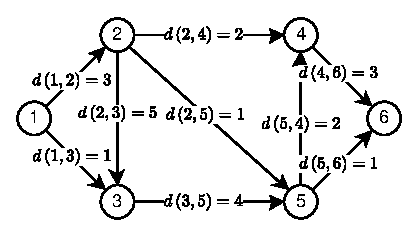
\includegraphics[width=\textwidth]{Chapter_I/3/1_3a.eps}
		\caption{}
	\end{subfigure}%
	%add desired spacing between images, e. g. ~, \quad, \qquad, \hfill etc.
	%(or a blank line to force the subfigure onto a new line)
	\qquad
	\begin{subfigure}[b]{0.33\textwidth}
		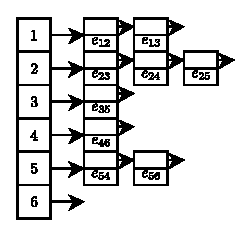
\includegraphics[width=\textwidth]{Chapter_I/3/1_3b.eps}
		\caption{}
	\end{subfigure}
	\caption{\textbf{Lista sąsiedztwa} \textbf{(a)} Graf skierowany $G = \left( V, E \right)$ z identyfikatorami węzłów $1-6$. Zamiast identyfikatorów łuków na krawędziach zostały naniesione wagi każdego z nich. \textbf{(b)} Listy sąsiedztw grafu $G$. Dla każdego węzła $v_{i} : i \in \left\{ 1, \ldots, 6 \right\}$ jest stworzona lista jednokierunkowa, której każdy element zawiera informację o pojedynczym łuku $e_{ij}$.}\label{fig:adjacencyList}
\end{figure}

Każdy taki łuk, oprócz swojej długości (dalej zwanej ogólniej: \textbf{kosztem}) będzie zatem posiadał dodatkowy atrybut, jednoznacznie wskazujący na węzeł, do którego prowadzi. Formalnie:

$v_{k} \in A \left ( i \right ) \Leftrightarrow \exists e_{ik} = \left( v_{i}, v_{k} \right) \in E $

Taką strukturę będziemy dalej nazywać zamiennie listą sąsiedztwa lub \textbf{incydencji} \footnote{Mówimy, że dwa wierzchołki są incydentne, jeżeli istnieje łącząca je krawędź.}.

\subsection{Pęki}

Na podobnym pomyśle, co listy sąsiedztwa, bazuje rozwiązanie z użyciem tzw. pęków. Tutaj także dla każdego węzła tworzyć będziemy "listę" węzłów, które są jego bezpośrednimi następnikami z tą różnicą, że te informacje będziemy zapisywać w jednej tablicy, nie na osobnych listach.

W niniejszym podrozdziale omówimy najbogatszą wersję reprezentacji z jednoczesnym wykorzystaniem \textbf{pęków wyjściowych} jak i \textbf{ wejściowych} (ang. \textit{Forward and Reverse Star Representation}), koncentrując się po kolei na pierwsze i drugiej części, które równie dobrze mogą stanowić samodzielne reprezentacje grafów.

\subsubsection{Pęki wyjściowe}

Załóżmy, że nasza reprezentacja grafu zawiera tablicę indeksowaną od $1$ do $ \left| V \right| $ - nazwijmy ją $vtab$. Stwórzmy drugą tablicę, która będzie konstruowana następująco:

dla każdego elementu tablicy $vtab$ o indeksie $vIdx$ (indeksy tej tablicy odpowiadają identyfikatorom wszystkich węzłów w grafie) będziemy chcieli, aby wartość, przechowywana w tej komórce, była równa minimalnemu indeksowi $aIdx$ w tablicy $atab$, dla którego element $atab \left[ aIdx \right] $ będzie zawierał informacje o łuku, wychodzącym z wierzchołka o identyfikatorze $vIdx$, zaś wartość $vtab \left[ vIdx+1 \right] $ będzie zawierała ostatni taki indeks, powiększony o jeden. Innymi słowy będziemy chcieli aby każdy element z tablicy $vtab$ zawierał informację o tym, od którego miejsca w tablicy $atab$ są przechowywane kolejno wszystkie informacje o łukach, wychodzących z węzła, przechowywanego w badanym elemencie pierwszej tablicy (rys. \ref{fig:forwardStarRepresentation}).

\begin{figure}[!htbp]
	\centering
	\begin{subfigure}[b]{0.5\textwidth}
		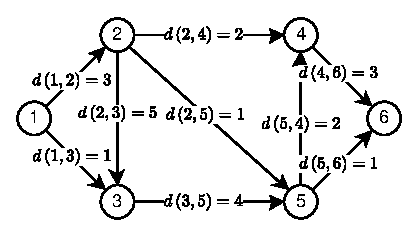
\includegraphics[width=\textwidth]{Chapter_I/4/1_4a.eps}
		\caption{}
	\end{subfigure}%
	\qquad
	\begin{subfigure}[b]{0.4\textwidth}
		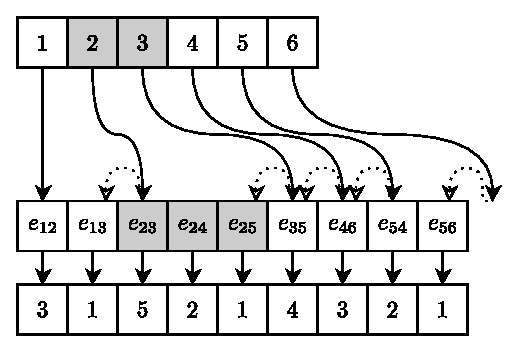
\includegraphics[width=\textwidth]{Chapter_I/4/1_4b.eps}
		\caption{}
	\end{subfigure}
	\caption{\textbf{Pęki wyjściowe} \textbf{(a)} Graf skierowany $G = \left( V, E \right)$ z identyfikatorami węzłów $1-6$. \textbf{(b)} Pęki łuków dla grafu $G$. Dla każdego węzła $v_{i} \in vtab$ element $ vtab \left[ i \right] $ zawiera indeks pierwszej, wychodzącej krawędzi z węzła $v_{i}$ w tablicy $atab$. Elementy w $atab$ są z kolei wskazaniami na odpowiednie krawędzie grafu.}\label{fig:forwardStarRepresentation}
\end{figure}

Na początku musimy stworzyć obie tablice, pierwszą ($vtab$) zainicjować samymi jedynkami (numer pierwszego indeksu łuku), zaś drugą pozostawić pustą - będziemy ją wypełniać w trakcie działania algorytmu. Następnie, iterując po tablicy z wierzchołkami $vtab$ odnajdujemy wszystkie łuki wychodzące z danego wierzchołka i wstawiamy dane takiej krawędzi (zakładamy, że są nimi identyfikatory łuków) do kolejnych elementów tablicy $atab$, jednocześnie zwiększając licznik $aIdx$. Gdy przeglądniemy wszystkie łuki wychodzące z pierwszego wierzchołka $v_{vIdx}$, wstawiamy do następnego elementu z tablicy $vtab$ ($vtab \left[ vIdx+1 \right] $) wartość licznika $aIdx$ - jest to najmniejszy indeks w tablicy $atab$, dla którego element $atab \left[ aIdx \right] $ będzie zawierał identyfikator łuku, wychodzącego z wierzchołka $v_{vIdx+1}$, a tym samym łatwo będziemy mogli policzyć, który element w tablicy zawiera ostatni łuk, wychodzący z wierzchołka poprzedniego (o indeksie $vIdx$). Algorytm kontynuujemy, dopóki nie przeglądniemy wszystkich elementów w tablicy $vtab$. W efekcie otrzymamy tablicę $atab$, której elementy będą posortowane rosnąco względem identyfikatorów wierzchołków, z których wychodzą, a każda para elementów $ \left( vtab \left[ i \right] , vtab \left[ i+1 \right] \right) $ będzie zawierać indeksy, dla których od $atab \left[ vtab \left[ i \right] \right] $ do $atab \left[ vtab \left[ i+1 \right] -1 \right] $ znajdują się łuki wychodzące z wierzchołka o indeksie $i$.

Jeżeli okaże się, że jakiś wierzchołek $v_{i}$ nie ma żadnych krawędzi wychodzących, wtedy $vtab \left[ i \right] = vtab \left[ i+1 \right] $, w szczególności $vtab \left[ 1 \right] = 1$ (pierwszy element, jako że indeksujemy od jedynki).

\begin{algorithm}[!htbp]
\DontPrintSemicolon
\KwData{$G= \left( V, E \right) $}
\KwResult{$atab \left[ 1 \ldots \left| E \right| \right] $}
\Begin{
	$aIdx \longleftarrow 1$\;
	$vtab \left[ 1 \ldots \left| V \right| \right] \longleftarrow aIdx$\;
	\For(\tcc*[f]{Dla każdego węzła w $vtab$}){$vIdx\in 1 \ldots \left| V \right| $}{
		\For{każdy łuk $e$, prowadząca z $v_{vIdx}$ do wierzchołka $\in A \left( vIdx \right) $}{
			$atab[aIdx] = e$\;
			$aIdx \longleftarrow aIdx + 1$\;
		}
	$vtab \left[ vIdx+1 \right] \longleftarrow aIdx$\; 
	}
}
\caption{CREATE-FORWARD-STAR-REPRESENTATION\label{alg:cfsr}}
\end{algorithm}


\subsubsection{Pęki wejściowe}

Mamy sytuację odwrotną: chcemy mieć możliwość szybkiego zidentyfikowania wszystkich wierzchołków wchodzących do danego węzła $v_{k}$. Algorytm jest taki sam jak w poprzednim przypadku z tą różnicą, że kolejność występowania łuków w tablicy $atab$ będzie inna - będą one występować w kolejności rosnących identyfikatorów węzłów, do których prowadzą, a nie mają początek. W obu przypadkach kolejność występowania krawędzi, wychodzących/prowadzących do tych samych wierzchołków nie ma znaczenia - w algorytmach wyszukiwania najkrótszych ścieżek, jeżeli zapytamy o dany węzeł to będziemy chcieli poznać wszystkich jego bezpośrednich następników/poprzedników, a nie tylko wybranego z nich.

\subsubsection{Pęki wejścia-wyjścia}

W pewnych przypadkach warto abyśmy dysponowali możliwością nie tylko szybkiego przeglądania tablic incydencji w poszukiwaniu następników, ale chcielibyśmy także mieć taką możliwość w odniesieniu do wszystkich poprzedników dowolnego węzła w sieci. Aby zrobić to oszczędnie, będziemy wykorzystywać fakt, że we wcześniejszych wersjach w tablicy $atab$ celowo trzymaliśmy tylko identyfikatory łuków, nie zaś ich wszystkie atrybuty (np. dla łuku o identyfikatorze $i$ o atrybutach: węzeł początkowy, końcowy oraz koszt, wartości te trzymalibyśmy w elementach osobnych tablic: $head \left[ i \right] $,  $tail \left[ i \right] $ oraz  $cost \left[ i \right] $). Jako podstawę dla naszego algorytmu weźmiemy pierwszą z omawianych reprezentacji, a więc zakładamy, że mamy tablice:

\begin{myitemize}
	\item $ vtab \left[ 1 \ldots \left| V \right| \right] $ - przechowującą informacje o łukach dla węzłów o identyfikatorach od $1$ do $ \left| V \right| $,
	\item $atab \left[ 1 \ldots \left| E \right| \right] $ - przechowującą krawędzie o identyfikatorach od $1$ do $ \left| E \right| $, posortowane rosnąco według identyfikatorów wierzchołków początkowych, gdzie dla każdego węzła $v_{k}$ wszystkie identyfikatory łuków wychodzących z tego węzła znajdują się w elementach od $atab \left[ vtab \left[ k \right] \right] $ do $atab \left[ vtab \left[ k+1 \right] -1 \right] $ włącznie
\end{myitemize}

i do nich chcemy dodać dwie nowe:

\begin{myitemize}
	\item $rtab \left[ 1 \ldots \left| V \right| \right] $ - analogicznie do $vtab$ przechowującą informacje o łukach dla węzłów o identyfikatorach od $1$ do $ \left| V \right| $ (dla reprezentacji odwróconej - \textit{Reverse Star Representation}),
	\item $mtab \left[ 1 \ldots \left| E \right| \right] $ - mapującą krawędzie o identyfikatorach od $1$ do $ \left| E \right| $.
\end{myitemize}

Druga z nich - $mtab$ - jest tablicą wejściową dla metody, opisanej w sekcji "Pęki wejściowe". Przechowuje ona w swoich kolejnych elementach indeksy tablicy $atab$ w taki sposób, aby ciąg \\ $atab \left[ mtab \left[ 1 \right] \right], atab \left[ mtab \left[ 2 \right] \right], \ldots, atab \left[ mtab \left[ \left| E \right| \right] \right] $ tworzył ciąg identyfikatorów łuków, które są posortowane rosnąco wedle wierzchołków wejściowych. Wówczas tablica $rtab$ razem z tablicą $mtab$ zachowuje się dokładnie tak samo jak druga para tablic.

\begin{figure}[!htbp]
	\centering
	\begin{subfigure}[b]{0.32\textwidth}
		\begin{subfigure}[b]{1\textwidth}
			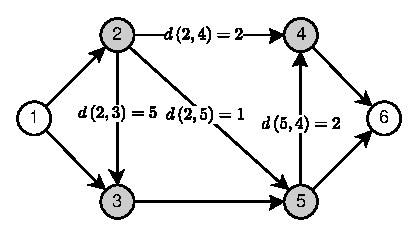
\includegraphics[width=\textwidth]{Chapter_I/5/1_5a.eps}
			\caption{}
		\end{subfigure}
		\begin{subfigure}[b]{1\textwidth}
			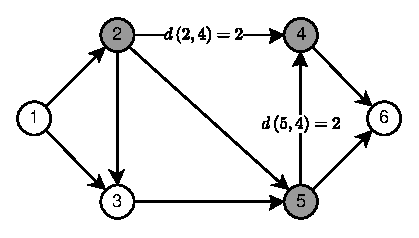
\includegraphics[width=\textwidth]{Chapter_I/5/1_5b.eps}
			\caption{}
		\end{subfigure}
	\end{subfigure}
	\qquad
	\begin{subfigure}[b]{0.50\textwidth}
		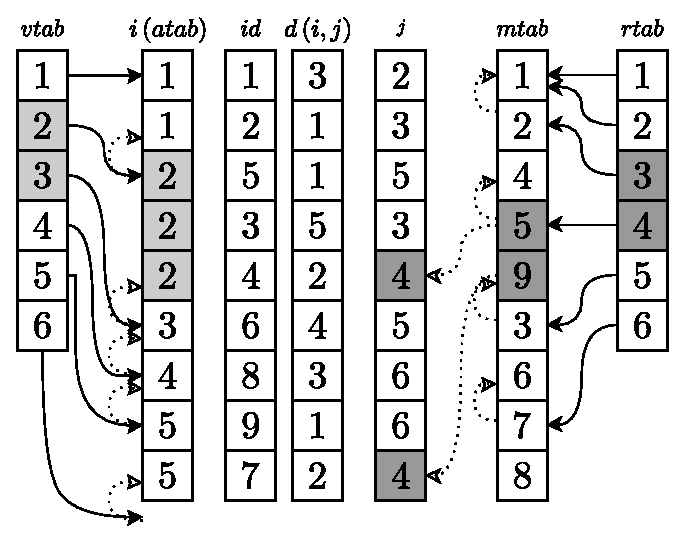
\includegraphics[width=\textwidth]{Chapter_I/5/1_5c.eps}
		\caption{}
	\end{subfigure}
	\caption{\textbf{Pęki wejścia-wyjścia} \textbf{(a)} Reprezentacja grafu $G = \left( V, E \right)$ z oznaczonymi następnikami węzła $v_{2}$. \textbf{(b)} Ten sam graf skierowany z oznaczonymi poprzednikami węzła $v_{2}$. \textbf{(c)} Graf przedstawiony w formie tablic.}\label{fig:forwardReverseStarRepresentation}
\end{figure}

Oczywiście taki sposób reprezentacji danych jest bardzo wrażliwy na wszelkie zmiany w strukturze sieci - każde usunięcie czy dodanie krawędzi powoduje konieczność aktualizacji wszystkich tablic, co jest bardzo pracochłonne, w porównaniu z reprezentacjami macierzowymi (gdzie taka operacja mogła być wykonana w czasie stałym) czy przy wykorzystaniu list sąsiedztwa (gdzie koszt dodawania krawędzi jest także stały, zaś koszt jej usunięcia to czas rzędu $ O \left( \left| E \right| \right) $). Taka reprezentacja natomiast pozwala nam na błyskawiczne - bo polegające na odjęciu wartości $vtab \left[ i \right] $ od $vtab \left[ i+1 \right] $ - policzenie \textbf{stopnia} wierzchołka $v_{i}$, a także uzyskać dostęp do wszystkich elementów $ v \in A \left( i \right) $ dla dowolnego wierzchołka $v_{i}$ w tym samym, liniowym, zależnym od ilości elementów w $A \left( i \right) $, czasie, jednocześnie przy zachowaniu stosunkowo małego - bo także liniowego - zapotrzebowania na pamięć (rys. \ref{fig:forwardReverseStarRepresentation}).

\subsection{Złożoność pamięciowa i czasowa}

Innym kryterium wyboru najodpowiedniejszego sposobu przedstawienia grafu jest ilość pamięci, jakiej wymagają implementacje poszczególnych rozwiązań. Dla obu implementacji macierzowych będą to wymagania rzędu $O \left( \left| V \right| \ldots \left| E \right| \right)$ lub $O \left( \left| V \right| \ldots \left| V \right| \right)$, odpowiednio dla macierzy incydencji i sąsiedztwa. Ile tak naprawdę z tej pamięci jest przez nas marnowanej najlepiej widać w przypadku, gdy mamy do czynienia z \textbf{grafem rzadkim} \footnote{graf, którego stosunek posiadanych krawędzi do ilości węzłów w danym grafie jest niewielki}, gdzie w takiej sytuacji większość macierzy jest wypełniona zerami (macierz rzadka). Stosując odpowiednie kodowanie, możemy wpłynąć na tą niepożądaną własność np. macierz incydencji, której elementy $a_{ij}$ posiadają tylko trzy wartości: $-1, 0, 1$ możemy przedstawić za pomocą dwóch macierzy, z której jedna - nazwijmy ją macierzą wyjścia - będzie zawierać jedynki na tych samych pozycjach, co poprzednia macierz, lecz w miejscach wystąpienia wartości ujemnej będzie miała wartość równą zero. Dla macierzy wejścia z kolei będziemy wstawiać jedynki w miejscach, gdzie uprzednio znajdowały się wartości przeciwne.

\begin{equation}
	a^{IN}_{ij}= \left\{ 
	\begin{array}{ll}
	1 & \textrm{jeżeli $a_{ij} = -1$,}\\
	0 & \textrm{w przeciwnym wypadku}
	\end{array} \right.
\end{equation}

\begin{equation}
	a^{OUT}_{ij}= \left\{ 
	\begin{array}{ll}
	1 & \textrm{jeżeli $a_{ij} = 1$,}\\
	0 & \textrm{w przeciwnym wypadku}
	\end{array} \right.
\end{equation}

Następnie zamieniamy każdą macierz na ciągi binarne długości $ \left| V \right| \ldots \left| E \right| $ każdy. Jest to prosta metoda na zgromadzenie potrzebnych nam informacji na jak najmniejszym fragmencie pamięci (jedna informacja - 1 bit), dodatkowo umożliwiająca nam bardzo szybkie przeszukiwanie takiej macierzy za pomocą operacji bitowych, a wykonanie kopii tak zgromadzonych danych to już nie koszt skopiowania wartości każdego elementu macierzy, a przepisanie jednej, potencjalnie olbrzymiej, liczby. Jednakże taka metoda wpływa tylko na obniżenie stałej i asymptotycznie nie daje żadnych widocznych różnic, jeżeli mówimy o złożoności pamięciowej, gdyż nadal pamiętamy $\left| V \right| \cdot \left| E \right|$ elementów.

W przypadku macierzy sąsiedztwa złożoność pamięciowa wynosi $O \left( \left| V \right| ^{2} \right) $, co nie powinno być dla nas zaskoczeniem, gdyż na obu osiach macierzy znajdują się wszystkie wierzchołki grafu. Oczywistym także jest, że zapotrzebowanie na pamięć będzie wzrastać im więcej informacji będziemy chcieć przechowywać w komórkach macierzy.

Dla samych list sąsiedztwa będziemy potrzebowali $O \left( \left| E \right| \right) $ pamięci, gdzie stała znowu może się różnić, w zależności od tego ile danych będziemy chcieli przechowywać w elementach list. Podczas tworzenia $ \left| V \right| $ list incydencji mamy zagwarantowane, że żadnego łuku nie dodamy dwa razy oraz, że wszystkie łuki w grafie zostaną do nich dodane (łuk z definicji ma tylko jeden początek i koniec, więc jeśli dany łuk $e \in A \left( i \right)$ dla węzła $v_{i}$ to na pewno nie należy do żadnego $A \left( j \right)$, gdzie $j \neq i$). Stąd elementów na wszystkich $ \left| V \right| $ listach sąsiedztwa jest dokładnie $ \left| E \right| $ elementów. Łącznie zatem, aby zaimplementować rozwiązania oparte na listach sąsiedztwa, potrzebujemy $ O \left( \left| V \right| + \left| E \right| \right)$ pamięci.

Mamy zatem:

~

\begin{savenotes}
	\begin{center}
		\begin{tabular}{ccccc}
			\hline
			& \multicolumn{2}{c}{Macierze} & \multicolumn{1}{c}{Listy} & \multicolumn{1}{c}{Pęki} \\
			& Incydencji & Sąsiedztwa & Sąsiedztwa & Wejścia-wyjścia \\
			\hline
			Potrzebna pamięć & $ O \left( \left| V \right| \cdot \left| E \right| \right) $  & $ O \left( \left| V \right| ^{2} \right)$ & $ O \left( \left| V \right| + \left| E \right| \right)$ & $ O \left( \left| V \right| + \left| E \right| \right)$ \\
			\hline
			Przegląd $v \in A \left( i \right) $ & $O \left( \left| E \right| + \left| A \left( i \right) \right| \cdot \left| V \right| \right)$ & $O \left( \left| V \right| \right) $ & $O \left( \left| A \left( i \right) \right| \right) $ & $O \left( \left| A \left( i \right) \right| \right) $ \\
			\hline
			Dodawanie krawędzi \footnote{W przypadku dodawania krawędzi znamy identyfikatory obu węzłów, z którymi połączony ma być dodawany łuk.} & $O \left( 1 \right)$ & $O \left( 1 \right) $ & $O \left( 1 \right) $ & $O \left( \left| V \right| + \left| E \right| \right) $ \\
			Dodawanie nowej krawędzi & $ O \left( \left| V \right| \cdot \left| E \right| \right) $ & $ O \left( 1 \right) $ & $O \left( 1 \right) $ & $O \left( \left| V \right| + \left| E \right| \right) $ \\
			Usuwanie krawędzi \footnote{Poza ostatnim przypadkiem, znany jest tylko identyfikator łuku i węzła, do którego dana krawędź prowadzi. Nie dotyczy to reprezentacji opartej na pękach wejścia-wyjścia, gdzie znajomość identyfikatora, jaki posiada łuk, daje nam dostęp do identyfikatorów obu węzłów, które ta krawędź łączy.} & $O \left( \left| V \right| \right)$ & $O \left( \left| V \right| \right) $ & $O \left( \left| E \right| \right) $ & $O \left( \left| V \right| + \left| E \right| \right)$ \\
			Trwałe usuwanie krawędzi & $ O \left( \left| V \right| \cdot \left| E \right| \right) $ & $ O \left( \left| V \right| \cdot \left| E \right| \right) $ & $O \left( \left| E \right| \right) $ & $O \left( \left| V \right| + \left| E \right| \right)$ \\
			Stopień wierzchołka & $O \left( \left| E \right| \right)$ & $O \left( \left| V \right| \right) $ & $O \left( \left| A \left( i \right) \right| \right) $ & $O \left( 1 \right) $ \\
		\end{tabular}
	\end{center}
\end{savenotes}

~

Jak widać rozdzieliliśmy operacje dodawania i usuwania elementów grafu, wyróżniając takie, które mają na celu tylko "zakryć" obecność danego elementu, bądź z powrotem przywrócić jego widoczność oraz na takie, których celem jest permanentna modyfikacja, przechowywanego w pamięci, grafu. Różnicę między tymi operacjami bardzo wyraźnie widać w przypadku korzystania z reprezentacji macierzowych grafu, gdzie "usunięcie" krawędzi możemy przeprowadzić w czasie zdecydowanie krótszym, niż byśmy mieli zmieniać rozmiar samych macierzy poprzez usuwanie/dodawanie elementów na którejkolwiek z ich osi. Chcąc "usunąć" z grafu daną krawędź wystarczy abyśmy zlokalizowali węzły, z którymi ma ona połączenie i w odpowiednich komórkach macierzy zamazali zapis o istniejącym połączeniu (założyliśmy, że w nasze grafy są skierowane tak więc znając łuk, który chcemy usunąć, mamy informację tylko o węźle, do którego dany łuk prowadzi - w obu przypadkach reprezentacji macierzowych zmusza nas to do dodatkowego przeszukania jednej z wybranych kolumn, w celu odszukania węzła, z którego łuk, który chcemy usunąć, wychodzi). Krawędź w grafie nadal będzie istnieć, lecz stanie się ona bezużyteczna, a dla algorytmów niezauważalna. Należy jednak tutaj podkreślić, że za takie traktowanie danych przyjdzie nam zapłacić, utrzymującym się na stałym poziomie, kosztem przeglądania macierzy w poszukiwaniu następników interesujących nas węzłów, zaś poza macierzowymi reprezentacjami różnice pomiędzy trwałym, a tymczasowym usuwaniem elementów nie ma żadnego wpływu na złożoność obliczeniową bez dodatkowych modyfikacji przedstawionych struktur.

~
\begin{center}
	\begin{tabular}{ccccc}
		\hline
		& \multicolumn{2}{c}{Macierze} & \multicolumn{1}{c}{Listy} & \multicolumn{1}{c}{Pęki} \\
		& Incydencji & Sąsiedztwa & Sąsiedztwa & Wejścia-wyjścia \\
		\hline
		Dodawanie węzła & $ O \left( \left| V \right| \cdot \left| E \right| \right) $ & $ O \left( 1 \right) $ & $O \left( 1 \right) $ & $O \left( \left| V \right| + \left| E \right| \right) $ \\
		Dodanie nowego  węzła & $ O \left( \left| V \right| \cdot \left| E \right| \right) $  & $ O \left( \left| V \right| ^{2} \right)$ & $ O \left( 1 \right)$ & $ O \left( \left| V \right| \right)$ \\
		Przysłonięcie węzła & $ O \left( \left| V \right| \cdot \left| E \right| \right) $  & $ O \left( \left| V \right| \right)$ & $ O \left( \left| E \right| \right)$ & $ O \left( \left| V \right| + \left| E \right| \right)$ \\
		Trwałe usunięcie węzła & $ O \left( \left| V \right| \cdot \left| E \right| \right) $  & $ O \left( \left| V \right| ^{2} \right)$ & $ O \left( \left| E \right| \right)$ & $ O \left( \left| V \right| + \left| E \right| \right)$ \\
	\end{tabular}
\end{center}

~

Poza takimi operacjami jak: dodawanie, usuwanie krawędzi grafu, wyznaczanie stopnia wierzchołka, jego następników możemy także chcieć na bieżąco modyfikować ilość węzłów, jakie znajdują się w grafie. Poniżej przedstawiono zestawienie czasów trwania wymienionych operacji dla wszystkich omówionych sposobów reprezentacji grafu. Podobnie jak w poprzednim przypadku, dla macierzy incydencji potrafimy wykonać operację "usuwania" węzła bez faktycznej zmiany rozmiarów tych macierzy, jednak w tym wypadku zysk z takiego postępowania jest niewielki, by wręcz nie powiedzieć: asymptotycznie żaden - podstawowym pomysłem na wymazanie informacji o danym węźle jest usunięcie wszystkich danych o łukach, które do niego prowadzą tak, aby węzeł przestał być osiągalny, lecz (jak pokazaliśmy wyżej) każdorazowa operacja samego wymazania informacji o pojedynczej krawędzi już kosztuje nas $O \left( \left| V \right| \right) $. W najgorszym przypadku musielibyśmy usunąć wszystkie krawędzie w grafie, co daje nam łącznie złożoność operacji tymczasowego usuwania węzła $O \left( \left| V \right| \cdot  \left| E \right| \right) $. 

Nieco lepsze rezultaty jesteśmy w stanie osiągnąć z macierzami sąsiedztw, gdyż w tym przypadku odnalezienie wiersza/kolumny z danym węzłem, który chcemy usunąć, jest równoznaczne z odnalezieniem wszystkich łuków, które do niego prowadzą i, gdybyśmy zignorowali konieczność zmiany rozmiaru całej macierzy (chcieli tylko ukryć jej elementy), to otrzymalibyśmy górne ograniczenie na złożoność tej operacji na poziomie $ O \left( \left| V \right| \right)$.

\begin{figure}[!htbp]
	\centering
	\begin{subfigure}[b]{0.5\textwidth}
		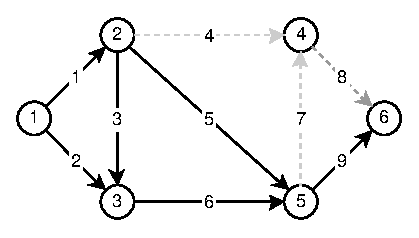
\includegraphics[width=\textwidth]{Chapter_I/6/1_6a.eps}
		\caption{}
	\end{subfigure}%
	\qquad
	\begin{subfigure}[b]{0.4\textwidth}
		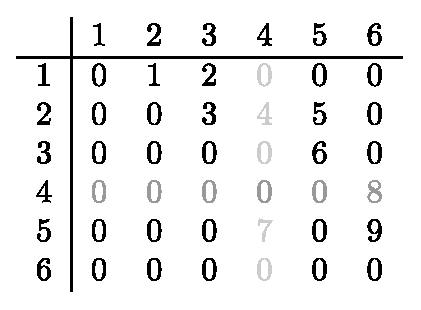
\includegraphics[width=\textwidth]{Chapter_I/6/1_6b.eps}
		\caption{}
	\end{subfigure}
	\caption{\textbf{Ukrycie węzła w macierzy sąsiedztwa} \textbf{(a)} Graf skierowany $G = \left( V, E \right)$. \textbf{(b)} Macierz sąsiedztwa dla grafu $G$. Chcemy ukryć w niej informację o $v_{4}$ tak, aby nie był on osiągalny z żadnego innego węzła w grafie. }\label{fig:adjacencyMatrixHideNode}
\end{figure}

Dla takiej koncepcji, dodanie na powrót węzła do grafu jest tylko kwestią dodania jakiegokolwiek łuku, który będzie łączył istniejący w sieci węzeł z tym, który chcemy dodać, więc koszty tej operacji będą identyczne, do dla dodawania krawędzi z poprzedniej tabeli.

W przypadku pozostałych dwóch struktur znowu nie odnotujemy żadnej zmiany - aby usunąć dany węzeł z list sąsiedztwa będziemy musieli odnaleźć wszystkie łuki, które prowadzą do usuwanego węzła, a na koniec usunąć całą listę jego sąsiedztwa, wraz z łukami, które się na niej znajdują. W najgorszym przypadku będzie od nas to wymagało przeglądnięcia wszystkich krawędzi, występujących w grafie, co uczynimy w czasie $ O \left( \left| E \right| \right) $. Dla pęków operacja usunięcia węzła jest jeszcze bardziej skomplikowana, gdyż nie istnieje w niej możliwość zaznaczenia konkretnego węzła, który chcielibyśmy ukryć, zaś jego usunięcie wymaga od nas odnalezienia obu zbiorów krawędzi (wychodzących z usuwanego węzła oraz do niego wchodzących), usunięcie ich z tablic, przechowujących o nich informacje (co uczynimy w czasie $ O \left( A \left( i \right) + A^{R} \left( i \right) \right) $ \footnote{Poprzez $A^{R} \left( i \right) $ oznaczać będziemy zbiór sąsiadów węzła $v_{i}$, lecz będą to węzły bezpośrednio ten węzeł poprzedzające, z których krawędzie prowadzą do tego węzła.}, zmiany ich rozmiarów ($ O \left( \left| E \right| \right) $), usunięcia danego węzła z dwóch pozostałych tablic, indeksowanych od $ 1 \ldots \left| V \right| $ (oraz zmiana ich rozmiarów - $ O \left( \left| V \right| \right) $)) oraz na końcu aktualizacji tych ostatnich ($ O \left( \left| V \right| \right) $) wraz z pomocniczą tablicą $mtab$, której rozmiar także trzeba zaktualizować ($ O \left( \left| E \right| \right) $).

\begin{figure}[!htbp]
	\centering
	\begin{subfigure}[b]{0.55\textwidth}
		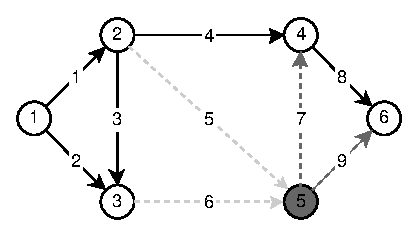
\includegraphics[width=\textwidth]{Chapter_I/7/1_7a.eps}
		\caption{}
	\end{subfigure}%
	\qquad
	\begin{subfigure}[b]{0.4\textwidth}
		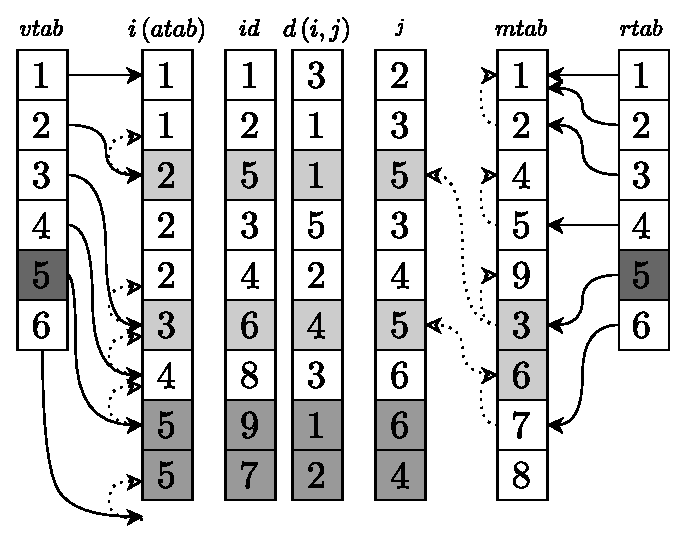
\includegraphics[width=\textwidth]{Chapter_I/7/1_7b.eps}
		\caption{}
	\end{subfigure}
	\caption{\textbf{Usunięcie węzła dla pęków wejścia-wyjścia} \textbf{(a)} Graf skierowany $G = \left( V, E \right)$. Usuwamy węzeł $v_{5}$ oraz wszystkie łuki wychodzące ($e_{7}, e_{9}$) i wchodzące do danego węzła ($e_{5}, e_{6}$). \textbf{(b)} Pęki z oznaczonymi łukami do usunięcia, wyznaczonymi odpowiednio w czasie $ O \left( A \left( 5 \right) \right)$ dla krawędzi wychodzących oraz $ O \left( A^{R} \left( 5 \right) \right)$ dla przychodzących. Węzeł, który należy usunąć wyznaczamy w czasie $ O \left( 1 \right)$. }
	\label{fig:forwardReverseStarRepresentationDeleteNode}
\end{figure}

\begin{figure}[!htbp]
	\ContinuedFloat
	\centering
	\begin{subfigure}[b]{0.4\textwidth}
		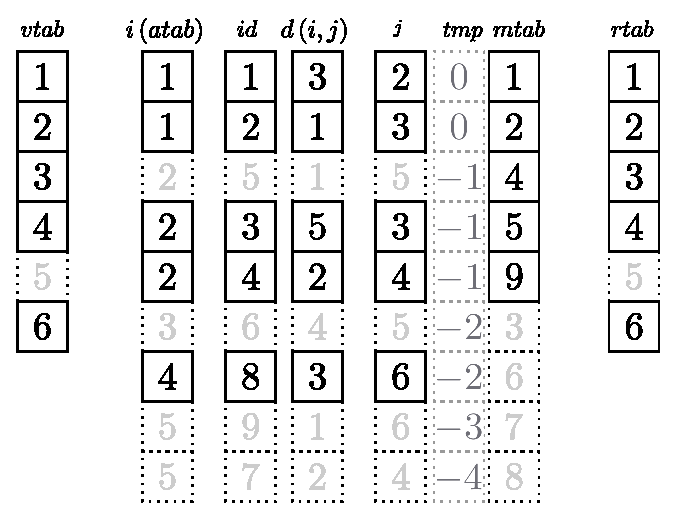
\includegraphics[width=\textwidth]{Chapter_I/7/1_7c.eps}
		\caption{}
	\end{subfigure}%
	\qquad
	\begin{subfigure}[b]{0.55\textwidth}
		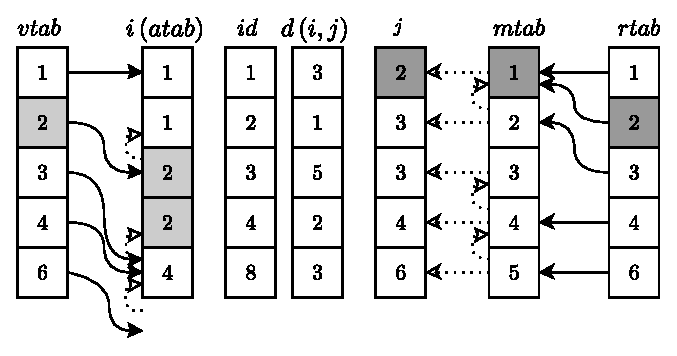
\includegraphics[width=\textwidth]{Chapter_I/7/1_7d.eps}
		\caption{}
	\end{subfigure}
	\caption{\textbf{(c)} Tablice z usuniętymi powiązaniami - po usunięciu chcianych elementów odtworzymy je w czasie liniowym. Rekonstrukcja związków, zachodzących między tablicami $vtab$, a $atab$ wymagać będzie przejścia przez ich wszystkie elementy, wyjąwszy krawędzie, wychodzące z ostatniego węzła, gdyż jego lista następników naturalnie kończy się wraz z końcem tablicy (po usunięciu wszystkich elementów tablice $vtab$ i $atab$ nadal będą prawidłowo posortowane). \textbf{(d)} Stan tablic po usunięciu węzła wraz z wszystkimi łukami. Odtworzenia własności tablicy $rtab$ oraz $mtab$ wymaga od nas większego nakładu pracy (ciąg wartości  \\ $j \left[ mtab \left[ 1 \right] \right], \ldots, j \left[ mtab \left[ \left| E \right| \right] \right] $ musi tworzyć ciąg niemalejący). W tym celu wprowadzamy pomocniczą tablicę, w której zapiszemy różnice indeksów elementów, jakie nastąpią w tablicy $j$ w trakcie usuwania krawędzi, a następnie aktualizujemy wszystkie elementy tablicy $mtab$ tak, aby $mtab \left[i \right] = mtab \left[i \right] + tmp \left[ mtab \left[ i \right] \right]$ (poza tymi, które wskazują na łuki, które będziemy usuwać - tutaj cztery ostatnie). \textbf{(d)} Sytuacja po usunięciu węzła $v_{5}$ i zaktualizowaniu wartości w tablicach. Szarym kolorem zaznaczono węzeł $v_{2}$ i powiązane z nim łuki.  }\label{fig:forwardReverseStarRepresentationDeleteNode1}
\end{figure}

W następnych rozdziałach spojrzymy już na sam problem najkrótszej ścieżki od strony zarówno formalnej jak i praktycznej - omówimy podstawowe własności problemu, zdecydujemy się na jeden ze, omówionych w powyższych rozdziałach, sposobów reprezentacji grafu, przedstawimy dodatkowe założenia, które ułatwią nam rozwiązanie problemu, jaki przed sobą postawiliśmy. Na koniec rozdziału - tak jak pisaliśmy na samym jego początku - przedstawimy krótko praktyczne zastosowanie zdobytej przez nas wiedzy w postaci algorytmu Bellmana-Forda.

\section{Problem najkrótszych ścieżek}
\label{sec:shortestPathProblem}

Omówiliśmy sposoby w jaki efektywnie możemy reprezentować dane, potrzebne nam do wyznaczenia najkrótszej ścieżki z punktu $v_{p}$ do węzła $v_{k}$ w skierowanym grafie z cyklami $G = \left( V, E \right)$, nie definiując przy tym formalnie samego problemu najkrótszej ścieżki, gdyż do tej pory, do opisu wszystkich reprezentacji grafu $G$, wystarczały nam intuicje, podparte prostą logiką. W dalszych rozważaniach będziemy opierać się o następujące oznaczenia i definicje:

\begin{myitemize}

\item \textbf{Ścieżką} od węzła $v_{p}$ do węzła $v_{k}$ będziemy nazywać każdą krawędź $e \in E$ w grafie $G = \left( V, E \right)$ taką, że ma ona swój początek w wierzchołku $v_{p} \in V$ i jest skierowana w stronę wierzchołka $v_{k} \in V$, gdzie ścieżka ta ma swój koniec. Z każdą ścieżką powiązana jest jej \textbf{waga} - dalej zwana również \textbf{kosztem} - $c_{pk}$, gdzie indeksy $p$ i $k$ odpowiadają indeksom węzłów: początkowego $v_{p}$ oraz końcowego $v{k}$, a którego wartość jest obliczana na podstawie, poniżej zdefiniowanej, \textbf{funkcji wagi}.

\item \textbf{Funkcja wagi} - jest funkcją, na podstawie której jest obliczany \textbf{koszt} danej ścieżki $e_{ij}$. W pseudokodach będziemy ją zwykle oznaczali przez $ d \left( v, u, \ldots \right) $, gdzie ostatni argument ("$\ldots$") oznacza, że \textbf{koszt} danej ścieżki może być zależny od wielu dodatkowych parametrów. My będziemy koszt każdej ścieżki $e_{ij}$ utożsamiać po prostu z jej długością i będziemy się do takiego kosztu odwoływać poprzez $c_{ij}$ (ang. \textit{cost}). Parametry funkcji $ d \left( v, u, c \right) $ będą kolejno oznaczały:

\begin{myitemize}

\item[v] - węzeł początkowy o indeksie $i$,
\item[u] - węzeł początkowy o indeksie $j$,
\item[c] - koszt $c_{ij}$ związany z łukiem $e_{ij}$, łączącym węzły $v$ i $u$.

\end{myitemize}


\item \textbf{Najkrótszą ścieżką} ze \textbf{źródła} $v_{p}$ do węzła $v_{k}$ nazywać będziemy takim zbiorem $P = \left \langle v_{0}, v_{1}, \ldots, v_{k} \right \rangle $, że suma kosztów $c_{ij}$ ścieżek jest najmniejsza:

\begin{equation}
\sum_{e_{ij} \in P^{'}} c_{ij} = minimum : e_{ij} \in P^{'} \Leftrightarrow v_{i},v_{j} \in P \: \wedge \: v_{i} \leadsto v_{j} = e_{ij} \ni E.
\end{equation}

gdzie przez $v_{i} \leadsto v_{j}$ będziemy oznaczać pojedynczą ścieżkę z węzła $v_{i}$ do węzła $v_{j}$. Wprowadzimy także zapis $v_{i} \overset{k}\leadsto v_{k}$, przez który będziemy rozumieć drogę złożoną z $k$ ścieżek, prowadzących od punktu $v_{i}$ do $v_{k}$ (użyty symbol "$*$"~ zamiast liczby ścieżek oznacza, że nie interesuje nas konkretna ich ilość, tylko fakt istnienia ścieżki o zadanych właściwościach - z danym punktem początkowym i końcowym). 

\item \textbf{Źródłem} $v_{S}$ będziemy nazywać węzeł, z którego rozpoczynamy wyszukiwanie najkrótszych ścieżek do wszystkich pozostałych węzłów w grafie i będzie to nasz podstawowy cel przy konstruowaniu wszystkich algorytmów, rozwiązujących problem najkrótszych ścieżek.

\end{myitemize}

\subsection{Reprezentacja problemu}
\label{sub:problemRepresentation}

Oprócz, omawianych już, własności naszej struktury oraz jej elementów składowych, takich jak koszt ścieżek $c_{ij}$, wspomnianych list sąsiedztwa, wprowadzimy także dodatkowe parametry dla węzłów, którymi będą:

\begin{myitemize}

\item \textbf{identyfikator węzła (ID)} jednoznacznie określa dany węzeł.

\item \textbf{poprzednik węzła (pred/$\Pi$)}, dalej zwany również jego \textbf{rodzicem}, który będzie determinował poprzedni węzeł na najkrótszej ścieżce (dla węzła $v_{i}$ będzie wyznaczał $v_{i-1}$ w $P = \left \langle v_{0}, v_{1}, \ldots, v_{i-1}, v_{i}, \ldots v_{k} \right \rangle $),

\item \textbf{waga najkrótszej ścieżki do węzła ($d \left( i \right) $)}, który dla węzła $v_{i}$ będzie przyjmował zawsze wartość najmniejszego znanego, kosztu przejścia ze źródła do tego węzła - dalej będziemy mówić o górnym ograniczeniu na koszt najkrótszej ścieżki, co okaże się równoważne (jeśli węzeł $v_{i}$ za wartość $ d \left( i \right) $ przyjmie $k$ to znaczy, że każda ścieżka $v_{S} \overset{*}\leadsto v_{i}$, aby być tą najkrótszą musi mieć łączny koszt nie większy niż $ d \left( i \right) $, czyli mniejszy lub równy $k$). Ponad to założymy, że dla każdego węzła $j$, do którego nie istnieje żadna ścieżka (w tym najkrótsza), bądź nie jest ona jeszcze znana, wartość $d \left( j \right) = \infty$ - wtedy dowolna ścieżka, która będzie nam pozwalała osiągnąć węzeł $j$ natychmiastowo stanie się najkrótszą ścieżką, do niego prowadzącą. Formalnie:

\begin{equation}
	d \left( i \right) \geqslant \delta \left ( s, i \right ) = \delta \left ( v_{s}, v_{i} \right ) = 
	\begin{cases}
	 \min \left\{ c \left( s,i \right ) : v_{s} \overset{*}\leadsto v_{i} \right\} & \text{ jeśli } \exists v_{s} \overset{*}\leadsto v_{i} \\ 
	 \infty & \text{ w przeciwnym przypadku }
	\end{cases}
\end{equation}

gdzie:

\begin{equation}
c \left( p,k \right ) = c \left( v_{p}, v_{k} \right ) = \sum_{e_{ij} \in P} c_{ij} \; : \; P = \left \langle v_{p}, v_{1}, \ldots, v_{k} \right \rangle 
\end{equation}\label{eq:sumCost}

\end{myitemize}

Do wszystkich atrybutów węzłów będziemy odwoływać się w dalszej części albo umieszczając jego nazwę w górnym indeksie, jak to robiliśmy do tej pory (np. $v{i}^{ID}$ oznaczał identyfikator węzła $i$ ), albo pisząc ją za operatorem kropki w przypadku, gdy górny indeks będzie potrzebny nam do czego innego (np. zapis $v_{i}^{ \left( k \right) }.\Pi$ będzie oznaczał $k$'tego rodzica \footnote{W sensie takim, że dla $k=1$ (domyślnie) wyrażenie $v_{i}^{ \left( k \right) }.\Pi$ oznacza rodzica podanego węzła, dla $k=2$ dziadka, dla $k=3$ pradziadka itd.} węzła $v_{i}$).

Aby efektywnie móc rozwiązywać problem najkrótszych ścieżek musimy przyjąć kilka założeń, które wynikają zarówno ze specyfikacji samego problemu, z przyjętego modelu (rzeczywistych sieci drogowych) oraz ograniczeń, jakie nakłada na nas konieczność reprezentacji wszystkich danych w sposób zrozumiały dla komputera.

Na samym początku należy wspomnieć o sposobie numerowania podstawowych elementów grafu $G = \left( V, E \right)$. Do tej pory milcząco zakładaliśmy, że każdy wierzchołek $v \in V$ w grafie $G$ ma przypisany swój własny, unikalny identyfikator, będący dodatnią liczbą całkowitą. Co więcej, identyfikatory te były przypisywane do tych wierzchołków w kolejności rosnącej ze skokiem o 1 tak, aby identyfikator ostatniego węzła równocześnie był liczbą wszystkich węzłów w grafie. Podobnie numerowaliśmy wszystkie krawędzie $e \in E$ - pozostaniemy przy tych oznaczeniach dla prostoty omawianego problemu, lecz nic nie stoi na przeszkodzie, by zamiast zwykłych tablic (bo temu właśnie ma służyć taka numeracja elementów grafu) wykorzystać bardziej złożone struktury, bądź \textit{tablice z haszowaniem}, które pozwoliłyby nam nazywać węzły dowolnie (mapując ich nazwy na liczby naturalne od $1$ do $ \left| V \right| $).

Bardziej restrykcyjnym założeniem o podobnym charakterze jest ograniczenie wartości wag wszystkich krawędzi (a co za tym idzie wag najkrótszych ścieżek w węzłach) do liczb całkowitych dodatnich. O ile jego obejście także nie stanowi większego problemu (wystarczy podnieść rząd wielkości wszystkich wartości tak, aby otrzymać liczby całkowite) to brak spełnienia tego warunku uniemożliwi nam efektywną konstrukcję pewnych wariantów algorytmów Dijkstry, które w dużej mierze opierają swoje działanie o te właśnie wartości (wspomniane algorytmy omówimy w rozdziale \ref{sec:dijkstraBuckets}). Dodatkowo w międzyczasie przemyciliśmy kolejne bardzo ważne założenie, które poczynimy - żadna z wag krawędzi w naszym grafie nie będzie mogła przybrać wartości ujemnej. Założenie to nie tylko jest słuszne z siecią drogową jako modelem, który sobie obraliśmy, lecz także bezpośrednio z niego wypływa inna własność, którą chcielibyśmy, aby miała nasza sieć - brak cykli o ujemnej długości tj. brak takich zamkniętych ścieżek, którymi da się przejść, a których koszt całkowity jest niedodatni ($ c \left( i, i \right) < 0 $, gdzie $v_{i}$ to odpowiednio "początek"~ i "koniec"~ cyklu). 

\begin{figure}[!htbp]
	\centering
	\begin{subfigure}[b]{0.45\textwidth}
		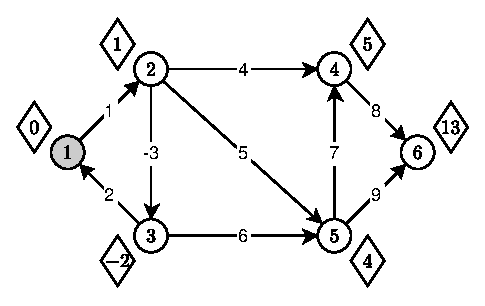
\includegraphics[width=\textwidth]{Chapter_I/8/1_8a.eps}
		\caption{}
	\end{subfigure}%
	\qquad
	\begin{subfigure}[b]{0.45\textwidth}
		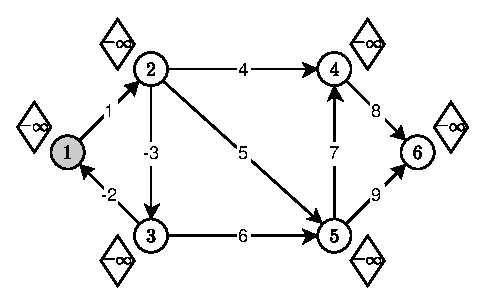
\includegraphics[width=\textwidth]{Chapter_I/8/1_8b.eps}
		\caption{}
	\end{subfigure}
	\caption{\textbf{Graf skierowany z ujemnymi wagami na krawędziach} \textbf{(a)} Węzeł $v_{1}$ jest źródłem, na krawędziach umieszczono ich wagi, a w rombach przy węzłach, do których prowadzą odpowiednio koszty najkrótszych ścieżek do tych węzłów ($d \left( 1 \right) = 0$). W samych węzłach umieszczono ich identyfikatory. Pomimo wystąpienia krawędzi $e_{23}$ o wadze $c_{23} < 0$ to długości najkrótszych ścieżek dla każdego z węzłów nadal są poprawnie wyliczone i przedstawiają faktyczny koszt najkrótszych ścieżek. \textbf{(b)} Wraz z pojawieniem się cyklu o ujemnej wadze ($v_{1} \leadsto v_{2} \leadsto v_{3} \leadsto v_{1} \leadsto \ldots$) wszystkie koszty w wierzchołkach stają się nieskończenie małe (z każdym kolejnym cyklem koszt dotarcia do węzłów w tym cyklu maleje, jednocześnie wpływając na koszt we wszystkich wierzchołkach, które są z tych węzłów osiągalne - dalej proces przebiega lawinowo, gdyż $- \infty + n = - \infty$). Oczywistym jest, że takie wyniki są dla nas bezwartościowe, gdyż informują co najwyżej o wystąpieniu w grafie ujemnego cyklu oraz o wierzchołkach, do których możemy dojść z jego wykorzystaniem.}\label{fig:negativeCycle}
\end{figure}

Jak pokazano na rysunku \ref{fig:negativeCycle}, za poprawną ścieżkę będziemy traktować tylko takie ścieżki, które nie zawierają w sobie cykli o ujemnej długości. Dodatkowo też za takie ścieżki będziemy uważać wszystkie, które zawierają cykl także o koszcie dodatnim (z analogicznego powodu). Załóżmy, że istnieje najkrótsza ścieżka $P = \left \langle v_{0}, v_{1}, \ldots, v_{k} \right \rangle $ taka, że $c \left( 0, k \right) = D$ i zawiera ona cykl dowolnej, niezerowej długości (powiedzmy $c = \left \langle v_{i}, v_{i+1}, \ldots, v_{j} \right \rangle $, gdzie $v_{i} = v_{j} $ oraz $c \left( i, j \right) \neq 0$). Nasza ścieżka zatem wygląda tak: $P = \left \langle v_{0}, v_{1}, \ldots, v_{i}, v_{i+1}, \ldots, v_{j}, \ldots, v_{k} \right \rangle $ (bez straty ogólności załóżmy, że cykl nie znajduje się na żadnym z końców ścieżki) i ma ona koszt $c \left( 0, k \right) = D$. Jeżeli chcielibyśmy usunąć teraz węzły cyklu od $v_{i+1}$ do $v_{j}$ to otrzymamy następującą ścieżkę: $P^{'} = \left \langle v_{0}, v_{1}, \ldots, v_{i}, v_{j+1}, \ldots, v_{k} \right \rangle $ o tym samym węźle początkowym i końcowym \footnote{Nie usuwamy pierwszego węzła cyklu, więc jeżeli cykl znajdowałby się na początku ścieżki to w oczywisty sposób węzeł $v_{p}$ na ścieżce $v_{p} \overset{*}\leadsto v_{k}$ nie uległby zmianie. Analogicznie w przypadku, gdyby cykl znajdował się na końcu tj. $P = \left \langle v_{0}, v_{1}, \ldots, v_{i}, v_{i+1}, \ldots, v_{j} \right \rangle $ i $v_{j}=v_{k}$, gdzie usunięcie cyklu spowodowałoby powstanie ścieżki  $P^{'} = \left \langle v_{0}, v_{1}, \ldots, v_{i} \right \rangle $. Pamiętając, że węzły $v_{i}$ oraz $v_{j}$ były odpowiednio początkiem i końcem cyklu $c$, a co za tym idzie: $v_{i} = v_{j} = v_{k} $.}, co poprzednia ścieżka (a więc "tą samą"~ ścieżkę), tyle że o zmienionym koszcie. Jeżeli usunęliśmy cykl o długości dodatniej, to nowa ścieżka będzie miała mniejszą wagę od ścieżki $P$, co czyni tą drugą dłuższą od $P^{'}$ - czyli ścieżka $P$ nie mogła być tą najkrótszą. Analogicznie możemy postępować dla cyklu o ujemnej długości, tyle że w tym przypadku zamiast usuwać cykle, będziemy je dodawać, by dojść do tej samej sprzeczności, co w poprzednio.

Z tego faktu dodatkowo wynika, że każda najkrótsza ścieżka może posiadać maksymalnie $\left| V \right| - 1$ składowych krawędzi - gdyby posiadała ich więcej, znaczyłoby to, że na ścieżce występuje cykl, a wykluczyliśmy już taką możliwość (nie zajmowaliśmy się cyklami długości zero, gdyż takie zawsze możemy eliminować z najkrótszych ścieżek).

Ostatnimi założeniami, jakie przyjmiemy, będą te związane z poprawną reprezentacją obliczeń, jakie będziemy wykonywać podczas wykonywania algorytmów (a które jedno już przedstawiliśmy). Jako, że dopuszczać będziemy sytuacje, w których dla danego węzła $v_{i}$ jego $v_{i}.d$ \footnote{$v_{i}.d \equiv v_{i}^{d} \equiv d \left( i\right)$} będzie się równać $- \infty$ albo $\infty$, konieczne jest zdefiniowanie operacji przy wykorzystaniu tych symboli nieoznaczonych. W związku z tym, będziemy przyjmować, że dla dowolnej liczby $n \neq \pm \infty$ zachodzić będą równości: $ a + \left( \mp \infty \right) = \left( \mp \infty \right) + a = \mp \infty$.

W dalszej części, przy omawianiu algorytmów, będziemy posługiwać się jedną z, przedstawionych wcześniej, reprezentacji grafu - w naszym przypadku będą to listy sąsiedztwa, gdyż w najbardziej naturalny (a zarazem najprostszy) sposób wyrażają one wszystkie własności, z jakich przyjdzie nam korzystać podczas konstruowania algorytmów wyszukiwania najkrótszych ścieżek.

\subsection{Podstawowe operacje}

Omówimy teraz podstawowe operacje, z których będziemy bardzo często korzystać w trakcie budowania kolejnych algorytmów wyszukujących najkrótsze ścieżki.

Jedną z takich operacji jest niewątpliwie procedura inicjalizująca graf, na którym dany algorytm będzie pracować. Jak wspomnieliśmy w poprzednich rozdziałach, w przypadkach, gdy nie istnieje najkrótsza ścieżka, bądź nie mamy informacji o takowej, która by prowadziła do danego węzła $i$, wtedy wartość parametru tego węzła $d \left( i \right) = \infty$ - przed rozpoczęciem działania algorytmu o ścieżkach nie wiemy nic, zatem każdy wierzchołek inicjalizujemy w ten sposób, dodatkowo upewniając się, że żaden z nich nie posiada informacji o swoim rodzicu (jako, że takie informacje posłużą nam później do odtworzenia znalezionych, najkrótszych ścieżek). Źródło $v_{S}$ - wierzchołek w grafie, od którego zaczniemy poszukiwania najkrótszych ścieżek - będzie miało ustawiony dystans ($d \left( S \right)$) na wartość równą zeru ("najkrótszą ścieżką" do węzła $v_{S}$ z węzła $v_{S}$ jest ścieżka długości zero - założyliśmy brak ujemnych cykli oraz brak jakichkolwiek krawędzi o takim koszcie).

\begin{algorithm}[!htbp]
\DontPrintSemicolon
\Begin{
	\For(\tcc*[f]{Dla każdego węzła w $vtab$}){$vIdx\in 1 \ldots \left| V \right| $}{
		$vtab \left[ vIdx \right].d \longleftarrow \infty$\; 
		$vtab \left[ vIdx \right].\Pi \longleftarrow \KwNull$\; 
	}
	$vtab \left[ s \right].d \longleftarrow 0$\; 
}
\caption{INIT-GRAPH $\left( G, s \right)$\label{alg:init-graph}}
\end{algorithm}

Dwa rozdziały temu wprowadziliśmy kilka nowych oznaczeń dla atrybutów węzłów, z których od tamtej pory mieliśmy korzystać. Mówiliśmy, że dla każdego węzła $v_{i}$ jego wartość $d \left( i \right) $ przyjmuje zawsze koszt równy najmniejszemu, znanemu kosztowi ścieżki, prowadzącej ze źródła do danego węzła , co formalnie możemy w skróconej formie wyrazić:

\begin{equation}
d \left( i \right) = \sum_{e_{jk} \in P} c_{jk} \rightarrow min\; : \; P = \left \langle e_{Sj^{ \left( 1 \right) }}, e_{j^{ \left( 1 \right) } j^{ \left( 2 \right) }}, \ldots, e_{j^{ \left( m \right) } i } \right \rangle
\end{equation}

gdzie $P$ jest zbiorem krawędzi dla istniejącej ścieżki $v_{S} \overset{m+1}\leadsto v_{i}$.

W czasie działania wszystkich algorytmów wyszukiwania najkrótszych ścieżek będziemy chcieli zachować tę własność, by w momencie zakończenia ich działania otrzymywać poprawne wyniki (czyli by $\forall v \in V \; d \left( i \right) = \delta \left( s, i \right)$). Aby to było możliwe, musimy wprowadzić kolejną operację, którą będziemy nazywać operacją relaksacji krawędzi. Przyjrzyjmy się sytuacji, która zobrazuje jej działanie.

\begin{figure}[!htbp]
	\centering
	\begin{subfigure}[b]{0.45\textwidth}
		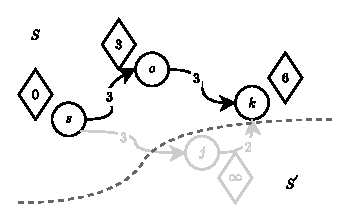
\includegraphics[width=\textwidth]{Chapter_I/9/1_9a.eps}
		\caption{}
		\label{fig:relaxEdges:a}
	\end{subfigure}%
	\qquad
	\begin{subfigure}[b]{0.45\textwidth}
		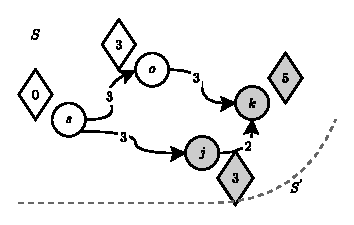
\includegraphics[width=\textwidth]{Chapter_I/9/1_9b.eps}
		\caption{}
		\label{fig:relaxEdges:b}
	\end{subfigure}
	\caption{\textbf{Relaksacja krawędzi} \textbf{(a)} Sytuacja przed dodaniem wierzchołka $v_{j}$ do zbioru wierzchołków o optymalnych wartościach $d \left( i \right) $, gdzie $i \in \left\{ i^{'} : v_{i^{'}} \in S \right\} $. \textbf{(b)} Dodanie do zbioru $S$ wierzchołka $v_{j}$ spowodowało powstanie nowej ścieżki $v_{s} \overset{*}\leadsto v_{k}$, której koszt jest mniejszy od dotychczasowej $v_{s} \leadsto v_{o} \leadsto v_{k}$ i w efekcie reorganizację najkrótszej ścieżki węzła $v_{k}$. Etykieta $ d \left( k \right)$ uległa zmniejszeniu, a $v_{k}.\Pi$ wskazuje teraz na węzeł $v_{j}$ (poprzednio $v_{o}$).}\label{fig:relaxEdges}
\end{figure}

Na rysunku \ref{fig:relaxEdges} przedstawiona jest sytuacja w trakcie działania pewnego algorytmu wyszukiwania najkrótszych ścieżek, gdzie wyszarzono wszystkie wierzchołki (oraz powiązane z nimi krawędzie), o których algorytm jeszcze nic nie wie (przyjmijmy, że zbiór tych wierzchołków będziemy oznaczać krótko jako $S^{'}$ - rys. \ref{fig:relaxEdges:a}), gdyż zaczął je przeglądać od danego węzła $v{S}$ - źródła. W tej chwili wszystkie atrybuty $d \left( i \right)$ węzłów nie należących do zbioru $S^{'}$ (nazwijmy go zbiorem $S$) mają wartości, odpowiadające kosztom najkrótszych ścieżek od źródła do każdego z nich (są optymalne) i jest to sytuacja, którą chcemy utrzymać. Przyjmijmy teraz, że do zbioru wierzchołków $S$ dołączamy wierzchołek $v_{j} \in S^{'}$ (jednocześnie go stamtąd usuwając - rys. \ref{fig:relaxEdges:b}). Po dodaniu wierzchołka $v_{j}$ widzimy, że do $v_{k}$ da się dojść krótszą ścieżką, niż to było przedstawione na rysunku \ref{fig:relaxEdges:a}, a zatem $d \left( k \right)$ nie jest już długością najkrótszej ścieżki dla tego węzła. Podobnie węzeł $v_{o} = v_{k}^{\Pi}$ nie należy już do zbioru węzłów, leżących na najkrótszej ścieżce $v_{S} \overset{*}\leadsto v_{k}$. Łatwo zauważyć, że jedyną możliwą alternatywą dla najkrótszej ścieżki do węzła $v_{k}$ jest przed chwilą powstała ścieżka, tak więc nowa wartość parametru $d \left( k \right) = min \left\{ d \left( o \right) + c_{ok}, d \left( k \right) \right\} $ \footnote{O tym, że tak jest w istcie przekonamy się w następnym rozdziale.}.

\begin{algorithm}[!htbp]
\DontPrintSemicolon
\Begin(\tcc*[f]{Oznaczenia węzłów zachowane z rysunku \ref{fig:relaxEdges}}){
	\If(\tcc*[f]{$d \left( j, k, \ldots \right)$ - funkcja wagi}){$ k.d > j.d + d \left( j, k \right)$} {
		$ k.d \longleftarrow j.d + d \left( u, k \right)$ \;
		$ k.\Pi \longleftarrow j$ \;
	}
}
\caption{RELAX $\left( j, k, d \right)$ \label{alg:relax}}
\end{algorithm}

Algorytm relaksacji wierzchołków sprawdza, czy nowo dodany wierzchołek zaburza, interesującą nas, własność grafu. Jeżeli nie to następne kroki są pomijane. W przeciwnym przypadku aktualizowane jest wskazanie na rodzica $d$ oraz wartość $d \left( i \right)$  dla wierzchołka, który tego wymaga. Metoda relaksacji przyjmuje trzy parametry, z którego dwa są wierzchołkami, a trzeci funkcją wagową krawędzi, którą zdefiniowaliśmy w podrozdziale \ref{sec:shortestPathProblem}.

Ostatnią operacją, którą chcielibyśmy móc wykonywać jest operacja przeglądania wierzchołków, które znajdują się na dowolnej najkrótszej ścieżce w grafie $G = \left( V, E \right)$, jako że sama informacja o długości takiej ścieżki nie zawsze okazuje się wystarczająca. Przy omawianiu dwóch poprzednich algorytmów na równi z operowaniem na atrybutach węzłów $d \left( i \right)$ pozwalaliśmy sobie zmieniać także atrybut, odpowiadający wskazaniu na rodzica danego węzła ($\Pi$), doprowadzając zawsze do sytuacji, w której rodzicem danego węzła, leżącego na najkrótszej ścieżce, zawsze był węzeł, który także na niej się znajdował, będąc jednocześnie o jedną krawędź bliżej źródła, od którego dana ścieżka się rozpoczynała. Innymi słowy dbaliśmy o to, by dla każdej najkrótszej ścieżki $ P = \left \langle v_{0}, v_{1}, \ldots, v{k} \right \rangle$ dla każdego $v_{i} : i \in \left\{ 1, \ldots, k \right\}$ zachodziła prawidłowość: $v_{i}.\Pi = v_{i-1}$ (dla $i = 0$ w oczywisty sposób $v_{0}.\Pi = \KwNull$), a zatem nasz algorytm, pozwalający nam na wypisanie po kolei węzłów na danej, najkrótszej ścieżce $v_{0} \overset{k} \leadsto v_{k}$, wyglądać mógłby dla przykładu tak:

\begin{algorithm}[!htbp]
\DontPrintSemicolon
\KwResult{Ścieżka, wypisane w kolejności od węzła docelowego do źródła.}
\Begin{
	\While{$ v.\Pi \neq \KwNull $} {
		Wypisz $v$ \;
		$  v \longleftarrow v.\Pi$ \;
	}
	Wypisz $v$ \;
}
\caption{WRITE-PATH $\left( v \right)$ \label{alg:writePAth}}
\end{algorithm}

gdzie na wejściu musielibyśmy podać węzeł, do którego ścieżkę chcemy wypisać, pamiętając, że będzie to ścieżka wypisana w odwrotnej kolejności i że nie jesteśmy w stanie wypisać najkrótszych ścieżek innych, niż te, które swój początek mają w źródle (zbiór wszystkich takich ścieżek tworzy swego rodzaju drzewo, którego korzeniem jest właśnie ten węzeł - rys. \ref{fig:shortestPathTree}).

\begin{figure}[!htbp]
	\centering
	\begin{subfigure}[b]{0.45\textwidth}
		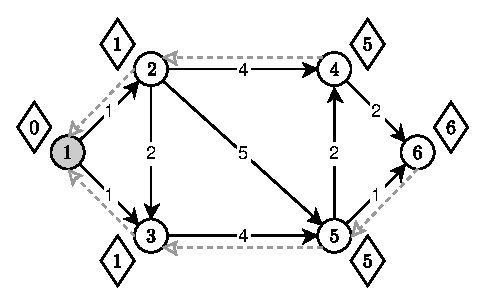
\includegraphics[width=\textwidth]{Chapter_I/10/1_10a.eps}
		\caption{}
	\end{subfigure}%
	\qquad
	\begin{subfigure}[b]{0.45\textwidth}
		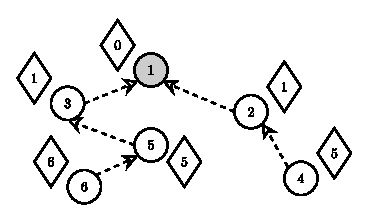
\includegraphics[width=\textwidth]{Chapter_I/10/1_10b.eps}
		\caption{}
	\end{subfigure}
	\caption{\textbf{Poddrzewo najkrótszych ścieżek} \textbf{(a)} Graf $G = \left( V, E \right)$ z obliczonymi odległościami najkrótszych ścieżek dla wszystkich węzłów, gdzie przerywanymi liniami zaznaczone są wskazania na poprzedników każdego z nich. W przypadku braku takiej krawędzi dla danego węzła $v$ zakładamy, że $v.\Pi = \KwNull$. \textbf{(b)} Poddrzewo grafu, zawierające najkrótsze ścieżki od źródła do wszystkich pozostałych węzłów w grafie $G$, w raz z ich kosztami.}\label{fig:shortestPathTree}
\end{figure}

Oczywiście nic nie stoi na przeszkodzie, byśmy zastosowali jedną z technik, by odwrócić kolejność takiego wypisywania (np. wpisać wyniki do kolejki FIFO, by później z niej odczytać wartości w kolejności od $v_{0}$ do $v_{k}$ czy też zastosować rekursję).

\subsection{Właściwości najkrótszych ścieżek}
\label{sub:shortestPathProperties}

Algorytmy, które będziemy omawiać w następnych rozdziałach, poza czerpaniem pomysłów na ich implementacje z wielu innych zagadnień informatycznych (jak się przekonamy), w głównej mierze oparte będą na właściwościach najkrótszych ścieżek, które przytoczymy w tym podrozdziale bez dowodów (Czytelnik może je wszystkie odnaleźć w dodatku TODO), wierząc, że pomoże się to skupić Czytelnikowi na samych algorytmach i dowodach ich poprawności, zwłaszcza, że zdecydowana większość właściwości najkrótszych ścieżek jest naturalna i łatwa do zrozumienia.

\begin{lemma}[Własność trójkąta]
Dla każdej krawędzi $e_{ij} \in E$ w zachodzi $ \delta \left( v_{k}, v_{j} \right) \leqslant \delta \left( v_{k}, v_{i} \right) + c_{ij}$.
\end{lemma}\label{lem:triangleInequality}

\begin{lemma}[Własność optymalnej podstruktury]
Jeśli w ważonym grafie skierowanym $ G = \left( V, E \right)$ z funkcją wagową $w: E \leftarrow \RR$ (w naszym przypadku wagi są utożsamiane z kosztem przejścia między jednym węzłem, a drugim, wyrażonym - bez straty ogólności - w liczbach naturalnych, gdyż zajmujemy się rzeczywistymi sieciami drogowymi, w których odległości między dowolnymi dwoma punktami mierzymy w całkowitych wielokrotnościach przyjętej jednostki długości) najkrótszą ścieżką z wierzchołka $v_{p}$ do $v_{k}$ jest ścieżka $P = \left \langle v_{p}, v_{p+1}, \ldots, v_{k} \right \rangle $ to dla każdych $i,j$ takich, że $p \leqslant i \leqslant j \leqslant k$ podścieżka $P_{ij} = \left \langle v_{i}, v_{i+1}, \ldots, v_{j} \right \rangle $ jest najkrótszą ścieżką z $v_{i}$ do $v_{j}$.
\end{lemma}\label{lem:optimalSubstructure}

\begin{lemma}[Własność braku ścieżki]
Jeśli nie istnieje ścieżka z $s$ do $v_{i}$ to zawsze $v_{i}.d = \delta \left( s, i \right) = \infty$
\end{lemma}\label{lem:noPath}

\begin{lemma}[Własność ścieżki z ujemnym cyklem]
Jeśli istnieje ścieżka $P = \left \langle v_{p}, v_{p+1}, \ldots, v_{k} \right \rangle $ z $v_{p}$ do $v_{i}$, na której znajduje się cykl o ujemnej wadze $P = \left \langle v_{i}, v_{i+1}, \ldots, v_{j} \right \rangle $, gdzie $p \leqslant i \leqslant j \leqslant k$ to zawsze $v_{k}.d = \delta \left( p, k \right) = - \infty$
\end{lemma}\label{lem:pathWithNegativeCycle}

\begin{lemma}[Własność górnego ograniczenia]
Dla każdego wierzchołka $v_{i} \in V$ zachodzi $ v_{i}.d \geqslant \delta \left( s , v_{i} \right)$, gdzie wartość $v_{i}.d$ monotonicznie maleje i w momencie osiągnięcia swojego dolnego ograniczenia $\delta \left( s , v_{i} \right)$ przestaje ulegać zmianie.
\end{lemma}\label{lem:costUpperBound}

\begin{lemma}[Własność zbieżności]
Jeśli w grafie ważonym $G = \left( V, E \right)$ istnieje najkrótsza ścieżka $P = \left \langle v_{p}, v_{p+1}, \ldots, v_{k-1}, v_{k} \right \rangle $ i w dowolnym momencie przed relaksacją krawędzi $e_{kk-1}$ zachodzi $ v_{k-1}.d = \delta \left( v_{p}, v_{k-1} \right)$ to po tej relaksacji $ v_{k}.d = \delta \left( v_{p}, v_{k} \right)$.
\end{lemma}\label{lem:convergenceProperty}

\begin{lemma}[Własność relaksacji dla ścieżki]
Jeśli $P = \left \langle v_{p}, v_{p+1}, \ldots, v_{k} \right \rangle $ jest najkrótszą ścieżką z $s = v_{p}$ do $v_{k}$ i wykonamy szereg relaksacji jej krawędzi w kolejności od $e_{pp+1}$ do $e_{k-1k}$ to $v_{k}.d$ będzie równe $ \delta \left( s, v_{k}\right)$ niezależnie od kolejności wykonywania pozostałych relaksacji.
\end{lemma}\label{lem:pathRelaxation}

\begin{lemma}[Własność podgrafu poprzedników]
Jeśli dla każdego węzła $v_{i}$ w grafie $G = \left( V, E \right)$ zachodzi $v_{i}.d = \delta \left( s, v_{i} \right)$ to podgrafem poprzedników grafu $G$ jest drzewo o korzeniu w węźle $s$ i krawędziach, będących odwzorowaniem wszystkich najkrótszych ścieżek w tym grafie.
\end{lemma}\label{lem:parentSubgraph}

\subsection{Algorytm Bellmana-Forda}

Ostatnim naszym krokiem w tym rozdziale będzie przedstawienie prostego algorytmu, wykorzystującego całą naszą, dotychczas zdobytą, wiedzę, do wyznaczenia najkrótszych ścieżek w zadanym, skierowanym grafie acyklicznym $G = \left( V, E \right)$ z nieujemnymi wagami na krawędziach. Algorytm, o którym będziemy mówić w tym rozdziale, jest oparty na właściwościach najkrótszych ścieżek, które omówiliśmy powyżej i bezpośrednio z nich wynika dowód jego poprawności, który także przytoczymy. Bardzo prostą ideą omawianego algorytmu jest wykonanie operacji relaksacji krawędzi w rundach aż "do skutku". Pod pojęciem rundy będziemy rozumieli przeprowadzenie takiej operacji dla każdej krawędzi w grafie dokładnie jeden raz, zaś wykonywanie rund będziemy powtarzać do momentu, w którym wartości $ d \left( i \right) $ każdego wierzchołka $V_{i}$ w grafie osiągną wartości równych rzeczywistym wagom najkrótszych ścieżek $v_{s} \overset{*}\leadsto v_{i}$ - dalej, dla zachowania prostoty, będziemy te wartości zapisywać w skrócie jako: $ \delta \left( s, i \right)$. Naszym celem zatem staje się już tylko znalezienie takiej minimalnej ilości rund, po których dla każdego wierzchołka $ v_{i} \in G $ zachodzi równość $ d \left( i \right) = \delta \left( s, i \right) $ (dla źródła $ s $). W tym momencie warto przypomnieć sobie, że w naszym modelu rzeczywistych sieci drogowych przyjęliśmy brak krawędzi, których koszt byłby mniejszy lub równy $ 0 $, a co za tym idzie najkrótsze ścieżki, które będziemy chcieli odnaleźć, nie będą składać się z więcej niż $ \left| V \right| - 1 $ elementów i przechodzić przez więcej niż  $ \left| V \right| -2 $ wierzchołków, nie wliczając to wierzchołka początkowego i końcowego - zwróciliśmy już uwagę na tę własność najkrótszych ścieżek pod koniec podrozdziału \ref{sub:problemRepresentation}.

\begin{algorithm}[!htbp]
\DontPrintSemicolon
\Begin{
	\For{$i = 1$ \emph{\KwTo} $ \left| V \right| - 1$}{
		\ForAll{$ \left( u, v \right) \in E$}{
		$RELAX \left( u, v \right)$ \;
		}
	}
	\ForAll{$ \left( u, v \right) \in E$}{
		\If{$ v.d > u.d + c_{uv}$}{
			\Return \KwFalse \;
		}
	}
	\Return \KwTrue \;
}
\caption{ BELLMAN-FORD $\left( G, s \right)$\label{alg:BellmanFord}}
\end{algorithm}

Powyżej została przedstawiona podstawowa wersja algorytmu Bellmana-Forda, której pesymistyczna złożoność, jeżeli chodzi o ilość wykonywanych operacji, da się w oczywisty sposób oszacować przez $ O \left( \left| V \right| \cdot \left| E \right| \right) $ - wykonujemy $ O \left( \left| V \right| \right) $ razy instrukcje $ \left( 3 \right) = \left( 4 \right) $, gdzie każda z nich wykonuje dokładnie $ \left| V \right| $ operacji \textsf{RELAX}. Druga pętla, którą widzimy, przegląda raz jeszcze wszystkie krawędzie w grafie, upewniając się, że nie można wykonać na którejkolwiek z nich dodatkowej relaksacji, czyli innymi słowy - czy nasz algorytm zakończył swoje działanie i dał poprawny wynik. Jeżeli po wykonaniu pierwszej z pętli znajdziemy taką krawędź $ \left( u, v \right) \in E $, że spełniony będzie warunek $ v.d > u.d + c_{uv}$ to niechybny znak, że w gafie, w którym szukaliśmy najkrótszych ścieżek od źródła $s$ do wszystkich pozostałych węzłów, występuje cykl o ujemnej długości. Do takiego wniosku dojdziemy, wykonując proste rozumowanie:

Załóżmy, że mamy w grafie cykl $C = \left \langle v_{0}, v_{1}, \ldots, v_{k} \right \rangle $, gdzie $ v_{0} = v_{k}$, a ponadto, że - mimo jego występowania - algorytm po wykonaniu drugiej pętli zwróci nam wartość pozytywną \textsf{\KwTrue} (czyli, że dla każdej krawędzi $ \left( u, v \right) \in E $ zaszła nierówność $ v.d \leqslant u.d + c_{uv}$ w tym i dla wszystkich krawędzi, należących do cyklu). Jak wspomnieliśmy w podrozdziale \ref{sub:problemRepresentation}, cyklem ujemnym nazywamy taką zamkniętą ścieżkę, po której jesteśmy w stanie przejść, a całkowity koszt przejścia po wszystkich krawędziach tego cyklu wynosi $ c \left( v_{0}, v_{k} \right) < 0 $ (nierówność \ref{eq:sumCost}). Dokładniej:

\begin{equation}
\exists C = \left \langle v_{0}, v_{1}, \ldots, v_{k} \right \rangle \; \wedge \; v_{0} = v_{k} \; \wedge \; \sum _{i=1}^{k} c \left( v_{i-1}, v_{i} \right ) = c \left( v_{0} , v_{k} \right) < 0 \Leftrightarrow C - \textrm{cykl o ujemnej długości}
\end{equation}

Kluczową dla naszego rozumowania okaże się nierówność $\sum _{i=0}^{k-1} c \left( v_{i}, v_{i+1} \right ) < 0$ oraz fakt, że z definicji cyklu $v_{0} = v_{k}$ gdzie $v_{0}, v_{k} \in C$. Z założenia, że algorytm Bellmana-Forda zwraca wartość \textsf{\KwTrue} mamy $\forall_{v_{i} \in C} \; v_{i}.d \leqslant v_{i-1}.d + c_{v_{i-1}v_{i}}$, gdzie sumując po $v_{1}, \cdots, v_{k} \in C$ otrzymujemy:

\begin{equation}
\sum _{i=1}^{k} v_{i}.d \; \leqslant \; \sum _{i=1}^{k} \left( v_{i-1}.d + c_{v_{i-1}v_{i}} \right) = \sum _{i=1}^{k} v_{i-1}.d + \sum _{i=1}^{k} c \left( v_{i-1}, v_{i} \right ) = \sum _{i=1}^{k} v_{i-1}.d + c \left( v_{0} , v_{k} \right)
\end{equation}.

Z własności cyklu: $v_{0} = v_{k}$ możemy wyprowadzić taki ciąg równości:

\begin{equation}
\sum _{i=0}^{k} v_{i}.d = v_{0}.d + \sum _{i=1}^{k-1} v_{i}.d + v_{k}.d = \sum _{i=1}^{k} v_{i-1}.d + v_{k}.d = v_{0}.d + \sum _{i=1}^{k} v_{i}.d
\end{equation}

zaś z obu wyprowadzeń w ostateczności otrzymujemy:

\begin{gather*}
\sum _{i=1}^{k} v_{i}.d \; \leqslant \; \sum _{i=1}^{k} v_{i-1}.d + c \left( v_{0} , v_{k} \right) \\
\sum _{i=1}^{k} v_{i}.d = \sum _{i=1}^{k} v_{i-1}.d \\
0 \; \leqslant \; c \left( v_{0} , v_{k} \right)
\end{gather*}

co stoi w sprzeczności z tym, że na naszej ścieżce znajduje się cykl o ujemnej długości ($ c \left( v_{0}, v_{k} \right) < 0 $). Widzimy więc, że algorytm Bellmana-Forda, podobnie zresztą jak wszystkie, omawiane w tej pracy algorytmy, nie radzi sobie z wyszukiwaniem najkrótszych ścieżek w grafach, gdzie występują cykle o długości ujemnej (jak pokazaliśmy na przykładzie \ref{fig:negativeCycle}).

Sam zaś algorytm można nieco usprawnić, by nie wykonywał niepotrzebnych operacji i przez to działał szybciej od swojego pierwowzoru. Nie są to jednak zmiany na tyle duże, by miały jakikolwiek wpływ na pesymistyczną złożoność algorytmu.

\begin{figure}[!htbp]
	\centering
	\begin{subfigure}[b]{0.24\textwidth}
		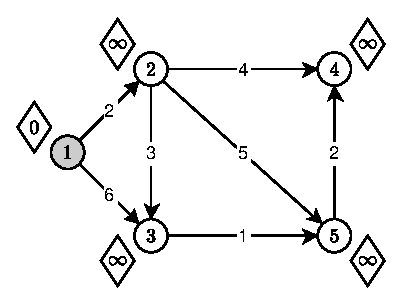
\includegraphics[width=\textwidth]{Chapter_I/11/1_11a.eps}
		\caption{}
	\end{subfigure}%
	\begin{subfigure}[b]{0.24\textwidth}
		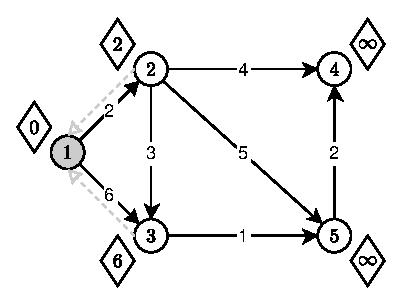
\includegraphics[width=\textwidth]{Chapter_I/11/1_11b.eps}
		\caption{}
	\end{subfigure}
	\begin{subfigure}[b]{0.24\textwidth}
		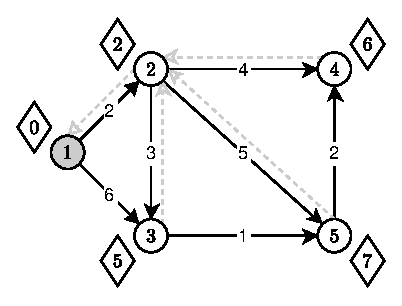
\includegraphics[width=\textwidth]{Chapter_I/11/1_11c.eps}
		\caption{}
	\end{subfigure}%
	\begin{subfigure}[b]{0.24\textwidth}
		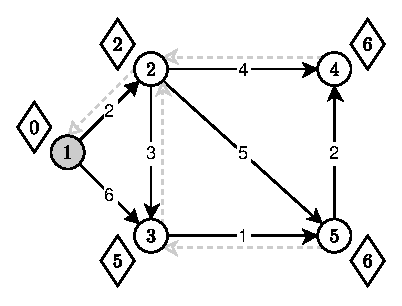
\includegraphics[width=\textwidth]{Chapter_I/11/1_11d.eps}
		\caption{}
		\label{fig:exampleBellmanFord:d}
	\end{subfigure}
	\caption{\textbf{Działanie algorytmu Bellmana-Forda} \textbf{(a)} Sytuacja po zainicjowaniu grafu $G = \left( V, E \right)$ przez \textsf{INIT-GRAPH} ze źródłem $v_{s}.id = 1$. \textbf{(b)} Warunek $ v.d > u.d + c_{uv} $ dla krawędzi $ \left( u, v \right) $ spełniony jest tylko dla krawędzi: $ \left( 1, 2 \right) $ i $ \left( 1, 3 \right) $ i dla tych węzłów ( $v_{2}$ i $v_{3}$ ) zostały zaktualizowani ich poprzednicy (zaznaczeni szarymi strzałkami) oraz etykiety $d$. Dla pozostałych algorytm nie wprowadził żadnych zmian w trakcie iterowania po wszystkich $ A \left( i \right) : i \in \left\{ 1, \ldots, 5\right\}$. \textbf{(c)} Przyjęliśmy kolejność iterowania po wszystkich łukach (pętla $3-4$) zgodną z kolejnością ponumerowania węzłów na rysunkach. Przyjmijmy ponadto rosnącą kolejność identyfikatorów węzłów, do której łuki prowadzą tj. podczas drugiej iteracji algorytm wykonuje operację \textsf{RELAX} na krawędziach w kolejności: $ \left( 1, 2 \right) $, $ \left( 1, 3 \right) $ (dla których relaksacja nie wprowadzi żadnych zmian), $ \left( 2, 3 \right) $ (zostaje zaktualizowany węzeł $v_{3}$ - jego wartość $d$ przyjmie długość odnalezionej, krótszej ścieżki oraz otrzyma nowego rodzica), $ \left( 2, 4 \right) $, $ \left( 2, 5 \right) $, \textbf{(d)} $ \left( 3, 5 \right) $ i $ \left( 5, 2 \right) $. Dla normalnej wersji algorytmu powinniśmy wykonać jeszcze 3 iteracje (z $ \left| V \right| - 1 $) po wszystkich krawędziach, jednak wprowadziliśmy modyfikację, która przerywa działanie algorytmu, jeżeli podczas pełnej iteracji nie nastąpi w grafie $G$ żadna zmiana.} \label{fig:exampleBellmanFord}
\end{figure}

\subsubsection{Usprawnienie algorytmu}

Pierwsze co możemy zauważyć to fakt, że jeśli uporządkujemy wszystkie krawędzie $e_{ij}$ względem pierwszego indeksu (czyli tak, aby kolejność przeglądania łuków w wierszach 3-4 była podyktowana przeglądanymi węzłami, z których dane łuki wychodzą) to możemy pomijać relaksacje tych wszystkich krawędzi, które wychodzą z węzła $v$, do którego jeszcze nie ma wyznaczonej ścieżki ($v.d = \infty$), gdyż warunek na jej wykonanie nigdy nie zajdzie ($ k.d > \infty + d \left( j, k \right)$). W wybranym przez nas sposobie prezentowania danych grafu (jako listy sąsiedztwa) taka kolejność przeglądania krawędzi jest naturalna (chcąc przejść przez wszystkie krawędzie w grafie będziemy kolejno przeglądać zawartość list $ A \left( i \right) : v_{i} \in G$). Dodatkowo - jak już zaznaczono na rysunku \ref{fig:exampleBellmanFord:d} - jeżeli w czasie wykonywania relaksacji wszystkich krawędzi w grafie nie nastąpi żadna zmiana to nie wystąpią one także podczas następnych iteracji głównej pętli algorytmu, a zatem możemy jej wykonanie przerwać, nie czekając aż wykona się ona dokładnie $ \left| V \right| - 1$ razy.

\subsubsection{Poprawność działania}

Dowód poprawności działania takiego algorytmu dla grafu $G = \left( V, E \right)$, który nie zawiera ujemnych cykli (dla których pokazaliśmy już, że omawiany algorytm nie działa) jest natychmiastowy, jeżeli powołamy się na odpowiednie własności najkrótszych ścieżek.

Z lematu \ref{lem:pathRelaxation} wiemy, że jeśli w grafie istnieje najkrótsza ścieżka $P = \left \langle v_{p}, v_{p+1}, \ldots, v_{k} \right \rangle $ i wykonamy dla jej krawędzi relaksację w odpowiedniej kolejności to $v_{k}.d$ będzie się równać $ \delta \left( s, v_{k} \right)$. Wiemy także, że każda najkrótsza ścieżka w grafie składać się może maksymalnie z $ \left| V \right| - 1 $ krawędzi. Z każdym nawrotem pętli głównej algorytmu Bellmana-Forda wykonywana jest relaksacja wszystkich krawędzi w grafie $G$, zaś pętla ta jest powtarzana dokładnie $ \left| V \right| - 1 $ razy. Podczas każdej $i$-tej iteracji w szczególności wykonamy relaksację dla wszystkich krawędzi na ścieżce $P$, a zwłaszcza dla $e_{pp+1}$ (w pierwszej iteracji), dla $e_{p+1p+2}$ i dla każdej następnej. W najgorszym przypadku, zależnym od faktycznej kolejności przeglądania krawędzi, ostatnią z nich na ścieżce $P$ będziemy relaksować w iteracji $k-p+1$ (w przypadku, gdy dla $k$ pierwszych $i$-tych iteracji $i = 1, 2, \cdots \left| V \right| - 1$ będziemy wykonywali relaksację tylko jednej krawędzi ze ścieżki $P$: łączącej węzeł $v_{p+ \left( i-1 \right)}$ z następnym węzłem $v_{p+ \left( i-1 \right) + 1}$), gdzie po ich wykonaniu $v_{k}.d = \delta \left( s, v_{k} \right)$. Analogiczne rozumowanie możemy przeprowadzić dla każdej najkrótszej ścieżki w grafie.

\section{Uwagi do rozdziału}

W tym rozdziale zapoznaliśmy Czytelnika z wszystkimi, podstawowymi pojęciami, które mają, przynajmniej taką mamy nadzieję, pomóc mu w pełniejszym zrozumieniu dalszej części, gdzie skupimy się na omawianiu kilkunastu algorytmów wyszukiwania najkrótszej ścieżki wraz z ich modyfikacjami, które pozwolą im na jeszcze szybsze działanie. Większą częścią z nich będą algorytmy oparte na podstawowym pomyśle holenderskiego informatyka Edsgera Dijkstry, którym poświęcimy cały następny dział. Podobnie jak algorytm Bellmana-Forda, będą one także służyły do znajdowania najkrótszej ścieżki z pojedynczego źródła w grafie bez ujemnych cykli, lecz tym razem nie będą mogły w nim występować krawędzie o takim koszcie ze względu na sposób realizacji algorytmu.